% Institute of Computer Science thesis template
% authors: Sven Laur, Liina Kamm
% last change Tõnu Tamme 09.05.2017
%--
% Compilation instructions:
% 1. Choose main language on line 55-56 (English or Estonian)
% 2. Compile 1-3 times to get refences right
% pdflatex bachelors-thesis-template
% bibtex bachelors-thesis-template
%--
% Please use references like this:
% <text> <non-breaking-space> <cite/ref-command> <punctuation>
% This is an example~\cite{example}.

\documentclass[12pt]{article}

  % A package for setting layout and margins for your thesis 
  \usepackage[a4paper]{geometry}
  
  %%=== A4 page setup ===
  %\setlength{\paperwidth}{21.0cm} 
  %\setlength{\paperheight}{29.7cm}
  %\setlength{\textwidth}{16cm}
  %\setlength{\textheight}{25cm}
  
  
  % When you write in Estonian then you want to use text with right character set
  % By default LaTeX does not know what to do with õäöu letters. You have to specify
  % a correct input and font encoding. For that you have to Google the Web     
  %
  % For TexShop under MacOS X. The right lines are 
  %\usepackage[applemac]{inputenc}
  %\usepackage[T1]{fontenc} %Absolutely critical for *hyphenation* of words with non-ASCII letters.
  %
  % For Windows and Linux the right magic lines are   
  % \usepackage[latin1]{inputenc}
  % \usepackage[latin5]{inputenc}
  %%\usepackage[utf8]{inputenc} %Package inputenc Error: Unicode char ´ (U+B4) not set up for use with LaTeX
  \usepackage[utf8x]{inputenc}
  \usepackage[T1]{fontenc} %Absolutely critical for *hyphenation* of words with non-ASCII letters.
  
  % Typeset text in Times Roman instead of Computer Modern (EC)
  \usepackage{times}
  
  % Suggested packages:
  \usepackage{microtype}  %towards typographic perfection...
  \usepackage{inconsolata} %nicer font for code listings. (Use \ttfamily for lstinline bastype)

  % Keeps floats in their place
  \usepackage{placeins}
  
  
  % Use package babel for English or Estonian 
  % If you use Estonian make sure that Estonian hyphenation is installed 
  % - hypen-estonian or eehyp packages
  %
  %===Choose the main language in thesis
  %\usepackage[estonian, english]{babel} %the thesis is in English 
  \usepackage[english, estonian]{babel} %the thesis is in Estonian
  
  
  % Change Babel document elements 
  \addto\captionsestonian{%
    \renewcommand{\refname}{Viidatud kirjandus}%
    \renewcommand{\appendixname}{Lisad}%
  }
  
  
  % If you have problems with Estonian keywords in the bibliography
  %\usepackage{biblatex}
  %\usepackage[backend=biber]{biblatex}
  %\usepackage[style=alphabetic]{biblatex}
  % plain --> \usepackage[style=numeric]{biblatex}
  % abbrv --> \usepackage[style=numeric,firstinits=true]{biblatex}
  % unsrt --> \usepackage[style=numeric,sorting=none]{biblatex}
  % alpha --> \usepackage[style=alphabetic]{biblatex}
  %\DefineBibliographyStrings{estonian}{and={ja}}
  %\addbibresource{bachelor-thesis.bib}
  
  
  % General packages for math in general, theorems and symbols 
  % Read ftp://ftp.ams.org/ams/doc/amsmath/short-math-guide.pdf for further information
  \usepackage{amsmath} 
  \usepackage{amsthm}
  \usepackage{amssymb}
  
  % Optional calligraphic fonts    
  % \usepackage[mathscr]{eucal}
  
  % Print a dot instead of colon in table or figure captions
  \usepackage[labelsep=period]{caption}
  
  % Packages for building tables and tabulars 
  \usepackage{array}
  \usepackage{tabu}   % Wide lines in tables
  \usepackage{xspace} % Non-eatable spaces in macros
  
  % Including graphical images and setting the figure directory
  \usepackage{graphicx}
  \graphicspath{{figures/}}
  
  % Packages for getting clickable links in PDF file
  %\usepackage{hyperref}
  \usepackage[hidelinks]{hyperref} %hide red (blue,green) boxes around links
  \usepackage[all]{hypcap}
  
  
  % Packages for defining colourful text together with some colours
  \usepackage{color}
  \usepackage{xcolor} 
  %\definecolor{dkgreen}{rgb}{0,0.6,0}
  %\definecolor{gray}{rgb}{0.5,0.5,0.5}
  \definecolor{mauve}{rgb}{0.58,0,0.82}
  
  
  % Standard package for drawing algorithms
  % Since the thesis in article format we must define \chapter for
  % the package algorithm2e (otherwise obscure errors occur) 
  \let\chapter\section
  \usepackage[ruled, vlined, linesnumbered]{algorithm2e}
  
  % Fix a  set of keywords which you use inside algorithms
  \SetKw{True}{true}
  \SetKw{False}{false}
  \SetKwData{typeInt}{Int}
  \SetKwData{typeRat}{Rat}
  \SetKwData{Defined}{Defined}
  \SetKwFunction{parseStatement}{parseStatement}
  
  
  % Nice todo notes
  \usepackage{todonotes}
  
  % comments and verbatim text (code)
  \usepackage{verbatim}
  
  
  % Proper way to create coloured code listings
  \usepackage{listings}
  % \lstset{ 
  %   %language=python,                % the language of the code
  %   language=C++,
  %   basicstyle=\footnotesize,        % the size of the fonts that are used for the code
  %   %numbers=left,                   % where to put the line-numbers
  %   %numberstyle=\footnotesize,      % the size of the fonts that are used for the line-numbers
  %   numberstyle=\tiny\color{gray}, 
  %   stepnumber=1,                    % the step between two line-numbers. If it's 1, each line 
  %                                    % will be numbered
  %   numbersep=5pt,                   % how far the line-numbers are from the code
  %   backgroundcolor=\color{white},   % choose the background color. You must add \usepackage{color}
  %   showspaces=false,                % show spaces adding particular underscores
  %   showstringspaces=false,          % underline spaces within strings
  %   showtabs=false,                  % show tabs within strings adding particular underscores
  %   frame = lines,
  %   %frame=single,                   % adds a frame around the code
  %   rulecolor=\color{black},		   % if not set, the frame-color may be changed on line-breaks within 
  %                                    % not-black text (e.g. commens (green here))
  %   tabsize=2,                       % sets default tabsize to 2 spaces
  %   captionpos=b,                    % sets the caption-position to bottom
  %   breaklines=true,                 % sets automatic line breaking
  %   breakatwhitespace=false,         % sets if automatic breaks should only happen at whitespace
  %   %title=\lstname,                 % show the filename of files included with \lstinputlisting;
  %                                    % also try caption instead of title
  %   keywordstyle=\color{blue},       % keyword style
  %   commentstyle=\color{dkgreen},    % comment style
  %   stringstyle=\color{mauve},       % string literal style
  %   escapeinside={\%*}{*)},          % if you want to add a comment within your code
  %   morekeywords={*,game, fun}       % if you want to add more keywords to the set
  % }
  
  
  % Obscure packages to write logic formulae and program semantics
  % Unless you do a bachelor thesis on program semantics or static code analysis you do not need that
  % http://logicmatters.net/resources/ndexamples/proofsty3.html <= writing type rules => use semantic::inference
  % ftp://tug.ctan.org/tex-archive/macros/latex/contrib/semantic/semantic.pdf
  % \usepackage{proof}
  \usepackage{semantic} 
  \setlength{\inferLineSkip}{4pt}
  \def\predicatebegin #1\predicateend{$\Gamma \vdash #1$}
  
  % If you really want to draw figures in LaTeX use packages tikz or pstricks
  % However, getting a corresponding illustrations is really painful  
  
  
  % Define your favorite macros that you use inside the thesis 
  % Name followed by non-removable space
  \newcommand{\proveit}{ProveIt\xspace}
  
  % Macros that make sure that the math mode is set
  \newcommand{\typeF}[1] {\ensuremath{\mathsf{type_{#1}}}\xspace}
  \newcommand{\opDiv}{\ensuremath{\backslash \mathsf{div}}\xspace} 
  
  % Nice Todo box
  \newcommand{\TODO}{\todo[inline]}
  
  % A way to define theorems and lemmata
  \newtheorem{theorem}{Theorem}


  \newcommand{\newlinespacer}{{%
    \newline
    \newline
  }}%\newcommand\newlinespacer


  %%% BEGIN DOCUMENT
  \begin{document}
  
  %===BEGIN TITLE PAGE
  \thispagestyle{empty}
  \begin{center}
  
  \large
  TARTU ÜLIKOOL\\
  Arvutiteaduse instituut\\
  Informaatika õppekava\\%[2mm]
  
  %\vspace*{\stretch{5}}
  \vspace{25mm}
  
  \Large Markus Peterson
  
  \vspace{4mm}
  
  \huge Dockeri konteinerite kaughaldus IoT seadmetes
  
  %\vspace*{\stretch{7}}
  \vspace{20mm}
  
  \Large Bakalaureusetöö (9 EAP)
  
  \end{center}
  
  \vspace{2mm}
  
  \begin{flushright}
   {
   \setlength{\extrarowheight}{5pt}
   \begin{tabular}{r l} 
    Juhendaja: Pelle Jakovits
   \end{tabular}
   }
  \end{flushright}
  
  %\vspace*{\stretch{3}}
  %\vspace{10mm}
  
  \vfill
  \centerline{Tartu 2018}
  
  %===END TITLE PAGE
  
  % If the thesis is printed on both sides of the page then 
  % the second page must be must be empty. Comment this out
  % if you print only to one side of the page comment this out
  %\newpage
  %\thispagestyle{empty}    
  %\phantom{Text to fill the page}
  % END OF EXTRA PAGE WITHOUT NUMBER
  
  
  %===COMPULSORY INFO PAGE
  \newpage
  
  %=== Info in English
  \newcommand\EngInfo{{%
  \selectlanguage{english}
  \noindent\textbf{\large Remote management of Docker containers in IoT devices}
  
  \vspace*{3ex}
  
  \noindent\textbf{Abstract:}
  
  \noindent
  The aim of this study is to create Cumulocity interface to remotely manage Docker containers on
  devices that are integrated into Cumulocity platform.
  Docker simplifies developing applications and deployment into production
  environment. It's benefits are also seen in IoT field where it is hard to maintain
  dependencies and new application versions on multiple devices. Cumulocity features device
  control, but currently has no interface to interact with Docker and it's containers. Using
  Cumulocity author creates device agent and webinterface that allows to interact with Docker
  through Cumulocity platform. This solution should support controlling lifecycle of containers,
  container configuration and container deployment.
  
  \vspace*{1ex}
  
  \noindent\textbf{Keywords:}\\
  IoT, Cumulocity, Node.js, AngularJS, Java, Docker
  %Layout, formatting, template
  
  \vspace*{1ex}
  
  \noindent\textbf{CERCS:}\\
  P170 (Computer science, numerical analysis, systems, control)
  
  \vspace*{1ex}
  }}%\newcommand\EngInfo
  
  
  %=== Info in Estonian
  \newcommand\EstInfo{{%
  \selectlanguage{estonian}
  \noindent\textbf{\large Dockeri konteinerite kaughaldus IoT seadmetes}
  \vspace*{1ex}
  
  \noindent\textbf{Lühikokkuvõte:} 
  
  %\noindent ...
  
  % \TODO{One or two sentences providing a basic introduction to the field, comprehensible to a scientist in
  % any discipline.}
  % \TODO{Two to three sentences of
  % more detailed background, comprehensible to scientists in related disciplines.}
  % \TODO{One sentence clearly stating the general problem being addressed by this particular
  % study.}
  % \TODO{One sentence summarising the main result (with the words ``here we show´´ or their equivalent).}
  % \TODO{Two or three sentences explaining what
  % the main result reveals in direct
  % comparison to what was thought to be the case previously, or how the main result adds to previous knowledge.}
  % \TODO{One or two sentences to put the results into a more general context.}
  % \TODO{Two or three sentences to provide a
  % broader perspective, readily
  % comprehensible to a scientist in any
  % discipline, may be included in the first paragraph
  % if the editor considers that the accessibility of
  % the paper is significantly enhanced by their inclusion.}

  \noindent
  Käesoleva bakalaureusetöö põhiteemaks on Cumulocity liidese loomine Dockeri konteinerite
  haldamiseks Cumulocityga integreeritud seadmetel üle võrgu. Docker lihtsustab oluliselt
  rakenduste arendamist
  ja kasutuselevõttu produktsioonis. Selle kasu on näha ka IoT valdkonnas, kus seadmete
  paljususe tõttu on keeruline hallata rakenduste sõltuvusi ja uute rakenduste versioonide
  kasutuselevõttu. Cumulocity platvorm pakub seadmete haldust, kuid praegusel hetkel ei ole
  leida liidest Dockeri konteinerite administreerimiseks. Kasutades Cumulocity platvormi
  luuakse liides IoT seadmetel Dockeri konteinerite haldamiseks. Täpsemalt peab liides
  võimaldama konteinerite elutsükli kontrollimist, konteinerite seadistamist ja konteinerite paigaldamist.
  
  \vspace*{1ex}
  
  \noindent\textbf{Võtmesõnad:}\\
  IoT, Cumulocity, Node.js, AngularJS, Java, Docker
  %Layout, formatting, template
  
  \vspace*{1ex}
  
  \noindent\textbf{CERCS:}\\
  P170 (Arvutiteadus, arvutusmeetodid, süsteemid, juhtimine (automaatjuhtimisteooria))
  
  \vspace*{8ex}
  }}%\newcommand\EstInfo
  
  
  %=== Determine the order of languages on Info page
  {\EstInfo}
  {\EngInfo}
  
  
  \newpage
  \tableofcontents
  
  
  % Remember to remove this from the final thesis version
  % \newpage
  % \listoftodos[Unsolved issues]
  % END OF TODO PAGE 
  
  
  \newpage
  \section{Sissejuhatus}
  
  % \TODO{What is it in simple terms (title)?}
  % \TODO{Why should anyone care?}
  % \TODO{What was my contribution?} 
  % \TODO{What you are doing in each section (a sentence or two per section)}
  
  % Tip: if it's hard for you to start writing, then try to split it to smaller parts, e.g. if the title is ``Type Inference for a Cryptographic Protocol Prover Tool'' then the ``What is it'' can be divided into ``what is type inference'', ``what is cryptographic protocol'' and ``what is the prover tool''. These three can also be split to smaller parts etc.

  \subsection{Sissejuhatus}

  % Asjade internet (inglise keeles Internet of Things) on igapäevaseadmetest koosnev infrastruktuur,
  % milles seadmed on ühendatud internetiga ja vahetavad üksteisega tihedalt andmeid ning integreeruvad
  % üksteisega. See on tänapäeval kujunenud üha trendikamaks tehnoloogiaks, kuna ettevõtted näevad seda
  % lisandväärtusena nii kasutajale kui ka ettevõttele endale.
  % \newlinespacer
  % IoT seadmed rikastavad süsteemi asukohapõhiste
  % andmetega, mis võimaldab kasutajal enda lähedal asuva seadme käest kõige täpsemat infot küsida. Näiteks
  % ilmateate rakenduste puhul saab lähimalt seadmelt küsida ilma kohta informatsiooni ja seade tagastab
  % tulemuse, mis on mõõdetud kasutaja vahetus läheduses.
  % \newlinespacer
  % Paljudest seadmetest koosnev süsteem muutub raskesti hallatavaks, kuna seadmete erinevuse tõttu
  % on ka viisid erinevad, mille abil seadmega ühenduda või mingeid operatsioone teostada.
  % Siin tuleb abiks Cumulocity, mille platvormiga on võimalik suvaline seade siduda läbi agendi,
  % mis seadmele installeeritakse. Agendid varieeruvad vastavalt seadmele ning funktsionaalsustele,
  % mida seade toetab. Seetõttu ei pruugi piisada mõni Cumulocity poolt valmis kirjutatud agentidest
  % vaid peab ise agendi arendama.

  % Asjade internet (inglise keeles Internet of Things) on igapäevaseadmetest koosnev infrastruktuur.
  % See on tänapäeval kujunenud üha trendikamaks tehnoloogiaks, kuna ettevõtted näevad seda
  % lisandväärtusena nii kasutajale kui ka ettevõttele endale.
  % Ettevõte jaoks tähendab see, et toode jõuab läbi suurema hulga seadmete rohkemate kasutajateni.

  % Asjade internet (inglise keeles Internet of Things) on igapäevaseadmetest koosnev infrastruktuur,
  % milles seadmed on ühendatud internetiga ja vahetavad üksteisega tihedalt andmeid ning integreeruvad
  % üksteisega. See on tänapäeval kujunenud üha trendikamaks tehnoloogiaks, kuna ettevõtted näevad seda
  % lisandväärtusena nii kasutajale kui ka ettevõttele endale.
  % \newlinespacer
  % IoT seadmed rikastavad süsteemi asukohapõhiste
  % andmetega, mis võimaldab kasutajal enda lähedal asuva seadme käest kõige täpsemat infot küsida. Näiteks
  % ilmateate rakenduste puhul saab lähimalt seadmelt küsida ilma kohta informatsiooni ja seade tagastab
  % tulemuse, mis on mõõdetud kasutaja vahetus läheduses.
  % \newlinespacer
  % Paljudest seadmetest koosnev süsteem muutub raskesti hallatavaks, kuna seadmete erinevuse tõttu
  % on ka viisid erinevad, mille abil seadmega ühenduda või administratiivseid operatsioone teostada.
  % Siin tuleb abiks Cumulocity, mille platvormiga on võimalik suvaline seade siduda läbi agendi,
  % mis seadmele installeeritakse. Agent on klientrakendus, mis platvormiga suhtleb.
  % Levinumatele seadmetele leiduvad agendid, mis on juba Cumulocity poolt valmis kirjutatud.
  % Tihtipeale nendest aga ei piisa, sest erinevate seadmete iseärasuste ja funktsionaalsuse
  % tõttu ei pruugi eelloodud agendid sobida. Seetõttu on Cumulocity pigem seadmete arendajatele
  % suunatud platvorm ning agendi loomine on jäetud arendajale.

  Asjade internet (inglise keeles Internet of Things) on igapäevaseadmetest koosnev infrastruktuur.
  See on tänapäeval üha rohkem populaarsemaks kujunev tehnoloogia, kuna ettevõtted näevad seda
  lisandväärtusena nii kasutajale kui ka ettevõttele endale. Seadmed asjade internetis on ühendatud
  internetiga ja vahetavad tihedalt andmeid ning integreeruvad üksteisega. Näitena saab tuua järgneva
  süsteemi.

  Matkaline jõuab külmal talvepäeval metsast koju ja soovib, et teda ootaks kodus ees kuum elektrisaun.
  Tal oli kogu retke jooksul käe peal nutikell, mis saab tema kehatemperatuuri jälgides aru, kui
  ta end läbi külmunult tunneb. Nutikell on samuti varustatud ka GPS seadmega ja tuvastab, kui
  kasutaja marsruudil koju on. Nende vaatluste järgi saadab nutikell kodus olevale eletrisaunale
  teate saun tööle panna.
  
  Tavapärane lahendus oleks, et nutikella ja elektrisauna vahel on ühendus ja
  need suhtlevad otse üksteisega. Antud süsteemi laiendamisel seadmete lisamisega,
  näevad süsteemid erinevate seadmete arvu puhul välja sellised:
  % Lisades süsteemi veel seadmeid, muutub nende omavaheline suhtlus
  % raskemaks, kuna igal seadmel peab olema ühendus teiste seadmetega.
  

  \begin{figure} [ht] %try to place the figure here (next option top of the page) 
  \begin{center}
  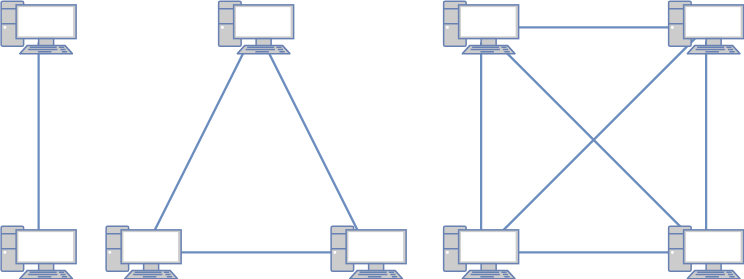
\includegraphics[width=0.8\textwidth]{decentralizedCommunication}
  \caption{Ühendused seadmete vahel tavapärases süsteemis}
  \label{fig:decentralizedCommunication}
  \end{center}
  \end{figure}
  \FloatBarrier
  
  
  Jooniselt \ref{fig:decentralizedCommunication} on näha, et seadmete lisamisel sellisesse
  süsteemi kasvab seadmetevaheline ühenduste arv kiiresti. 
  Seetõttu on kasulik kaasata süsteemi keskseade, mis koondab endasse informatsiooni seadmete kohta
  ja teab, kuidas nendega suhelda. Teised seadmed saavad üksteisega suhtlemise asemel suhelda
  keskseadmega, mis võtab info saatjalt vastu ja edastab selle saaja kätte.
  Läbi keskseadme on seadmed paremini hallatavad, kuna on võimalik monitoorida seadmetel
  toimuvat.
  Sellist lahendust nimetatakse tsenraliseeritud süsteemiks, mida illustreerib joonis
  \ref{fig:centralizedCommunication}.

  \begin{figure} [ht] %try to place the figure here (next option top of the page) 
  \begin{center}
  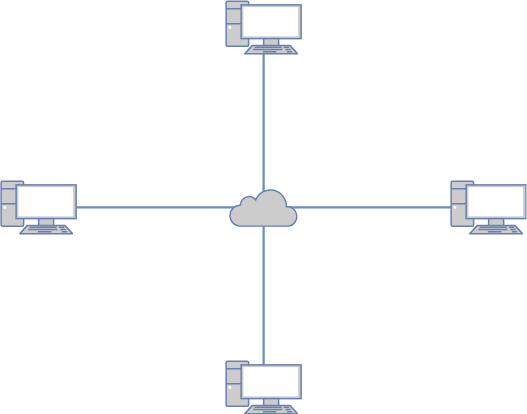
\includegraphics[width=0.6\textwidth]{centralizedCommunication}
  \caption{Ühendused seadmete vahel tsentraliseeritud süsteemis}
  \label{fig:centralizedCommunication}
  \end{center}
  \end{figure}
  \FloatBarrier
  
  Asjade interneti seadmete paremaks ühendamiseks, integreerimiseks ja haldamiseks loodi
  Cumulocity, mis töötab kui keskseade nende vahel. Cumulocity platvorm võimaldab luua
  paljudest erinevatest seadmetest koosnevaid süsteeme. Platvorm on eelkõige suunatud
  seadmete loojatele või rakenduste arendajatele, mistõttu tuleb luua sõltuvalt seadmest
  vastav liides platvormiga integreerumiseks. Selline geneerilisus lubab luua
  seadmele erivõimalustega funktsionaalsusi.

  Seadme halduse juures möödapääsmatuks osaks on tarkvara haldus ja selle uuendamine.
  Enamasti igal rakendusel on sõltuvused, mis peavad olema installitud, et rakendus
  korrektselt töötaks. Asjade interneti seadmete paljususe tõttu on see mahukas töö.
  Seetõttu on kasulik kasutada Dockerit, mis on virtualiseerimistehnoloogia, mis
  konteinerdab rakenduse koos sõltuvuste ja konfiguratsiooniga.
  Dockeri eeliseks on ka väiksem ressursikasutus kui tavapärastel
  virtualiseerimistehnoloogiatel, kuna Docker kasutab sama kernelit nagu host masina
  kernel~\cite{DockerDocOverview}.
  Integreerides
  Dockeri Cumulocity platvormi, saab kontrollida seadmetel töötavaid rakendusi
  ning neid kergelt uuendada.
  
  % Selline geneerilisus lubab arendajal luua seadmele erivõimalustega rakendusi, mis 
  % Selline geneerilisus lubab arendajal luua seadmele erivõimalustega funktsionaalsusi,






  \subsection{Lahendus}
  % Eesmärk on luua liides Cumulocity platvormi seadmetel töötavate Dockeri süsteemipiltide ja
  % konteinerite haldamiseks. 
  Pragusel hetkel ei ole leida lahendust, mis ühendaks omavahel Cumulocity platvormi
  ja Dockeri. Töö eesmärk on luua Cumulocity platvormi liides, mis lihtustaks Cumulocity platvormiga
  integreeritud seadmetel töötava tarkvara
  haldust kasutades Dockerit. Selle eeliseks on tarkvara paigutamine eelpakendatud
  modulaarsetesse tarkvarapakettidesse ehk süsteemipiltidesse, mida saab lihtsasti liigutada
  ning käivitada seadmes, millesse on Docker installitud. Süsteemipildi
  käivitamisel tehakse sellest konteiner, milles pakendatud tarkvara töötab
  isoleeritult~\cite{DockerDocOverview}.
  Kasutaja peab saama näha platvormi veebikeskkonnas seadmetel
  olevaid süsteemipilte ja konteinereid. Lisaks peab saama süsteemipilte kustutada ja uusi
  alla laadida. Konteinereid peab saama käivitada, peatada ja kustutada. Samuti peab nägema
  hetkel aktiivseid konteinereid.

  Liides luuakse kahes osas. Cumulocity veebiliidese moodul seadmete peal töötava
  Dockeri informatsiooni näitamiseks ning konteinerite ja süsteemipiltide haldamiseks
  luuakse Javascriptis kasutades Angular.js raamistikku. Teine osa on Cumulocity agent,
  mis vahendab infot Cumulocity platvormi ja seadmel töötava Dockeri tarkvara vahel.
  See luuakse Javas ja põhineb Cumulocity Bitbucketi
  repositooriumist pärit näitekoodil~\cite{cumulocityExamplesRepository}.

  Lõpptulemuseks on agentrakendus ja veebiliidese moodul, mis on vabavaralised ehk igaüks võib
  vaadata ja kopeerida koodi enda kasutamise huvides. See võib olla abiks praegustele
  arendajatele, et lihtsustada asjade interneti seadmete tarkvara haldust või aitab
  tutvuda Cumulocity platvormiga.


  \subsection{Ülevaade}
  % \noindent
  % 2. peatükk - Cumulocity tutvustus - tutvustab, kuidas Cumulocity sisemiselt töötab
  % \newline\noindent
  % 3. peatükk - Dockeri tutvustus - tutvustab Dockeri süsteemipilte ja konteinereid
  % \newline\noindent
  % 4. peatükk - Praktiline osa - kirjeldab agentrakenduse ja veebiliidese loomist
  Ülejäänud lõputöö struktuur on järgnev.
  Teine peatükk tutvustab lähemalt Cumulocityt ja selle sisemist tööpõhimõtet. Kolmas peatükk
  räägib virtualiseerimistehnoloogiast Docker, selle süsteemipiltidest ja konteineritest
  ning kuidas neid läbi Dockeri käsurea hallata. Neljas peatükk kirjeldab nõudeid loodavale
  Cumulocity liidesele, arhitektuurist, kuidas liides toimib, ja liidese loomisest endast
  ning lõpuks testitakse liidese vastavust püstitatud nõuetele. Viimane peatükk võtab
  lõputöö kokku.




  % Internet of Things (IoT) ehk asjade internet on igapäevaseadmetest koosnev infrastruktuur,
  % milles seadmed vahetavad üksteisega tihedalt andmeid ning integreeruvad üksteisega,
  % mis koos loovad parema kasutajakogemuse. Näiteks saavad kasutajad küsida andmeid lähedal asuvatelt
  % seadmetelt ümbritseva keskkonna temperatuuri kohta, mis võimaldab saada tegeliku temperatuuri väärtuse
  % kasutaja asukohas.

  % definitsioonid
  % teema kas on populaarne, miks
  % miks ta kasulik on

  % töö eesmärk
  % töökäik




  
  
  
  
  \newpage
  \section{Cumulocity tutvustus} 
  
  
  \subsection{Üldtutvustus}
  
  Cumulocity on peamiselt IoT seadmete integreerimiseks ja haldamiseks
  suunatud platvorm, mis ühendab seadmed ühisesse süsteemi
  ja võimaldab seadmetel suhelda üksteisega. Samuti lihtsustab see seadmetelt andmete kogumist,
  nende kontrollimist, konfigureerimist ja pakub
  reaalajalist logimist ning seadmete monitoorimist~\cite{CumulocityConceptsInterfaceingDevices,
  CumulocityConceptsDomainModel}.
  Seadme registreerimine platvormi toimub Cumulocity
  agendi jooksutamisel seadmel ning seejärel tuleb seade aksepteerida platvormis endas. Agent on
  programm, mis töötab seadmel ja suhtleb Cumulocity REST API-liidesega ja teeb end kättesaadavaks
  platvormile.
  Agent määrab, milliseid operatsioone on võimalik selle seadmega teha ning milliseid andmeid see
  seade enda kohta saadab.
  \newlinespacer
  Cumulocity platvormi veebiliides on sama paindlik. Veebiliidest on võimalik laiendada AngularJS-l
  põhinevate moodulitena, mis võimaldab kohandada kasutajaliidese elemente seadme seisundi ja
  andmete kuvamiseks ning lisada interaktiivseid kasutajaliidese elemente operatsioonide välja
  kutsumiseks.
  Cumulocity on selleks valmistanud ka cumulocity-tools nimelise teegi,
  mis tagab uue mooduli baaskoodi ja teeb saadavaks Cumulocity põhifunktsioonide teegi, mille abil
  on Cumulocity platvormi REST API-liidesega kergem suhelda. Tagatud on ka kujundus, et moodulid
  sarnased välja näeksid.
  \newlinespacer
  Paindlikus on see, mis võimaldab paljudel seadmetel Cumulocity platvormiga integreeruda. Tuntumate
  seadmete nagu näiteks Arduino, Raspberry Pi, Tinkerforge ja Kontron jaoks on loodud agendid, mida
  saab edasi arendada vastavalt vajadusele. Leidub ka Windowsile, Linuxile ja MacOSile mõeldud agente.
  \newlinespacer
  Cumulocity platvorm on üles ehitatud tenantite (eesti keeles üürnik) peale.
  Tenant kujutab endast kasutajate grupi üksust, läbi mille on võimalik platvormiga integreeruda.
  Sellised üksused on üksteisega seotud läbi puu struktuuri, mis tähendab, et
  igal tenantil on ülem, kellest see tenant tuletatud on, välja arvatud üks tenant.
  Selleks on juurtenant, mis on kuulub ettevõttele. Ülemtenantil on õigus alluvate
  tenantite haldamiseks enda õiguste piires. Tenantitel on samad õigused,
  mis nende ülemtenantil, kui ülemtenant pole teisiti määranud ja õiguseid
  kärpinud~\cite{CumulocityUsersGuideAdministration}.
  Tenantile määratud õigustest sõltub, mis selles tenantis on võimalik teha.


  
  \subsection{Põhirakendused}
    

  Cumulocity tenantis on esialgselt kolm põhirakendust, milledeks on
  administratsiooni, kopiti ja seadmehaldus rakendus.
  
  Administratsiooni rakenduse abil on võimalik lisada kasutajaid ja rolle
  ning neid eemaldada; hallata tenanti rakendusi, nende seadistusi,
  konfiguratsioone ning andmete säilitamise reegleid; tenanti logi vaatamine;
  failide lisamine, alla laadmine ja kustutamine. Failide lisamise abil saab
  üles laadida uue veebiliidese mooduli zip failina. Põhirakendustes uusi 
  mooduleid kasutada ei saa. Selleks tuleb neid kloonida administratsiooni rakenduse
  abil ja kasutada uusi mooduleid kloonitud rakendustes.
  Administratsiooni rakenduse esilehte on näha joonisel \ref{fig:cumulocityAdministration}.
  
  \begin{figure} [ht] %try to place the figure here (next option top of the page) 
  \begin{center}
  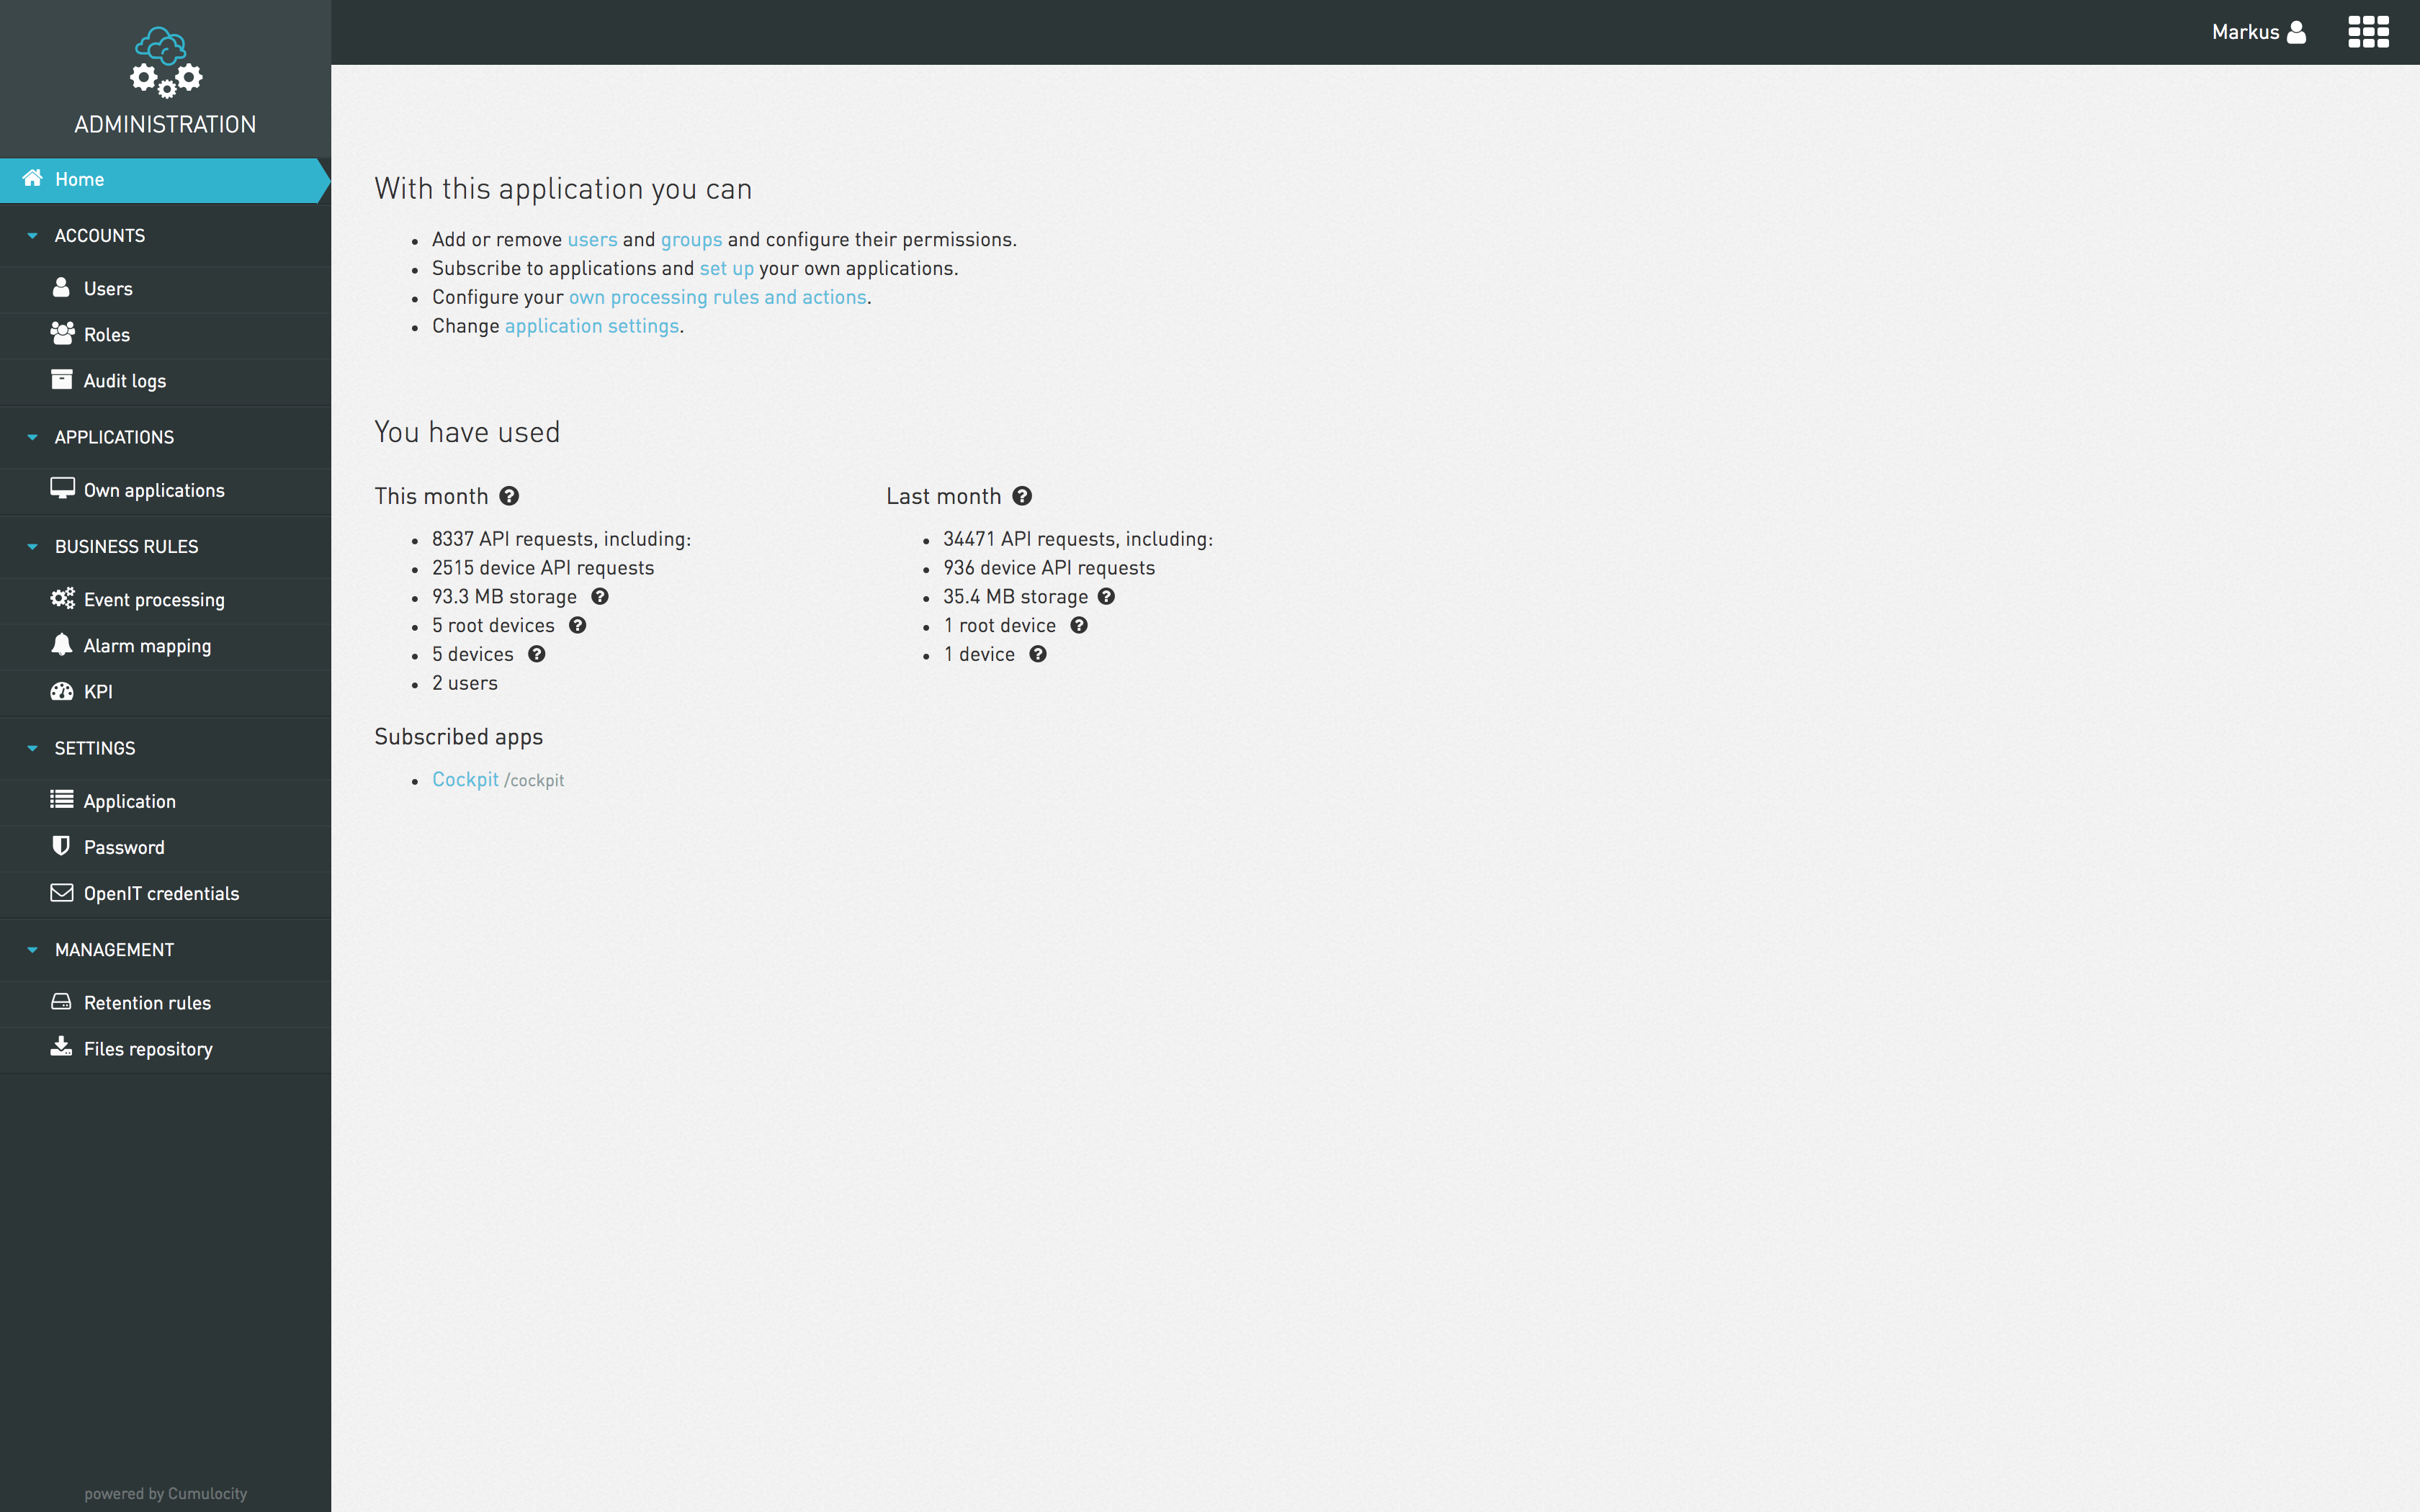
\includegraphics[width=1\textwidth]{cumulocityAdministration}
  \caption{Cumulocity administratsiooni rakendus}
  \label{fig:cumulocityAdministration}
  \end{center}
  \end{figure}

  \FloatBarrier

  Kokpiti rakendus võimaldab saada kiiret ülevaadet kogu platvormi kohta.
  Võimalik korraga vaadata kõiki alarme ning neid hallata; luua raporte,
  neid kloonida ja kustutada; tenanti mõõtetulemusi lisada, kustutada ja visualiseerida.
  Võimalus luua esipaneele ning neid kohandada komponentidega. See võimaldab kuvada
  ülevaatlikku informatsiooni kõikide seadmete kohta. Komponente on võimalik
  valida paljude eeldefineeritute seast või juurde arendada.
  Kokpiti rakenduse esilehte on näha joonisel \ref{fig:cumulocityCockpit}.

  \begin{figure} [ht] %try to place the figure here (next option top of the page) 
  \begin{center}
  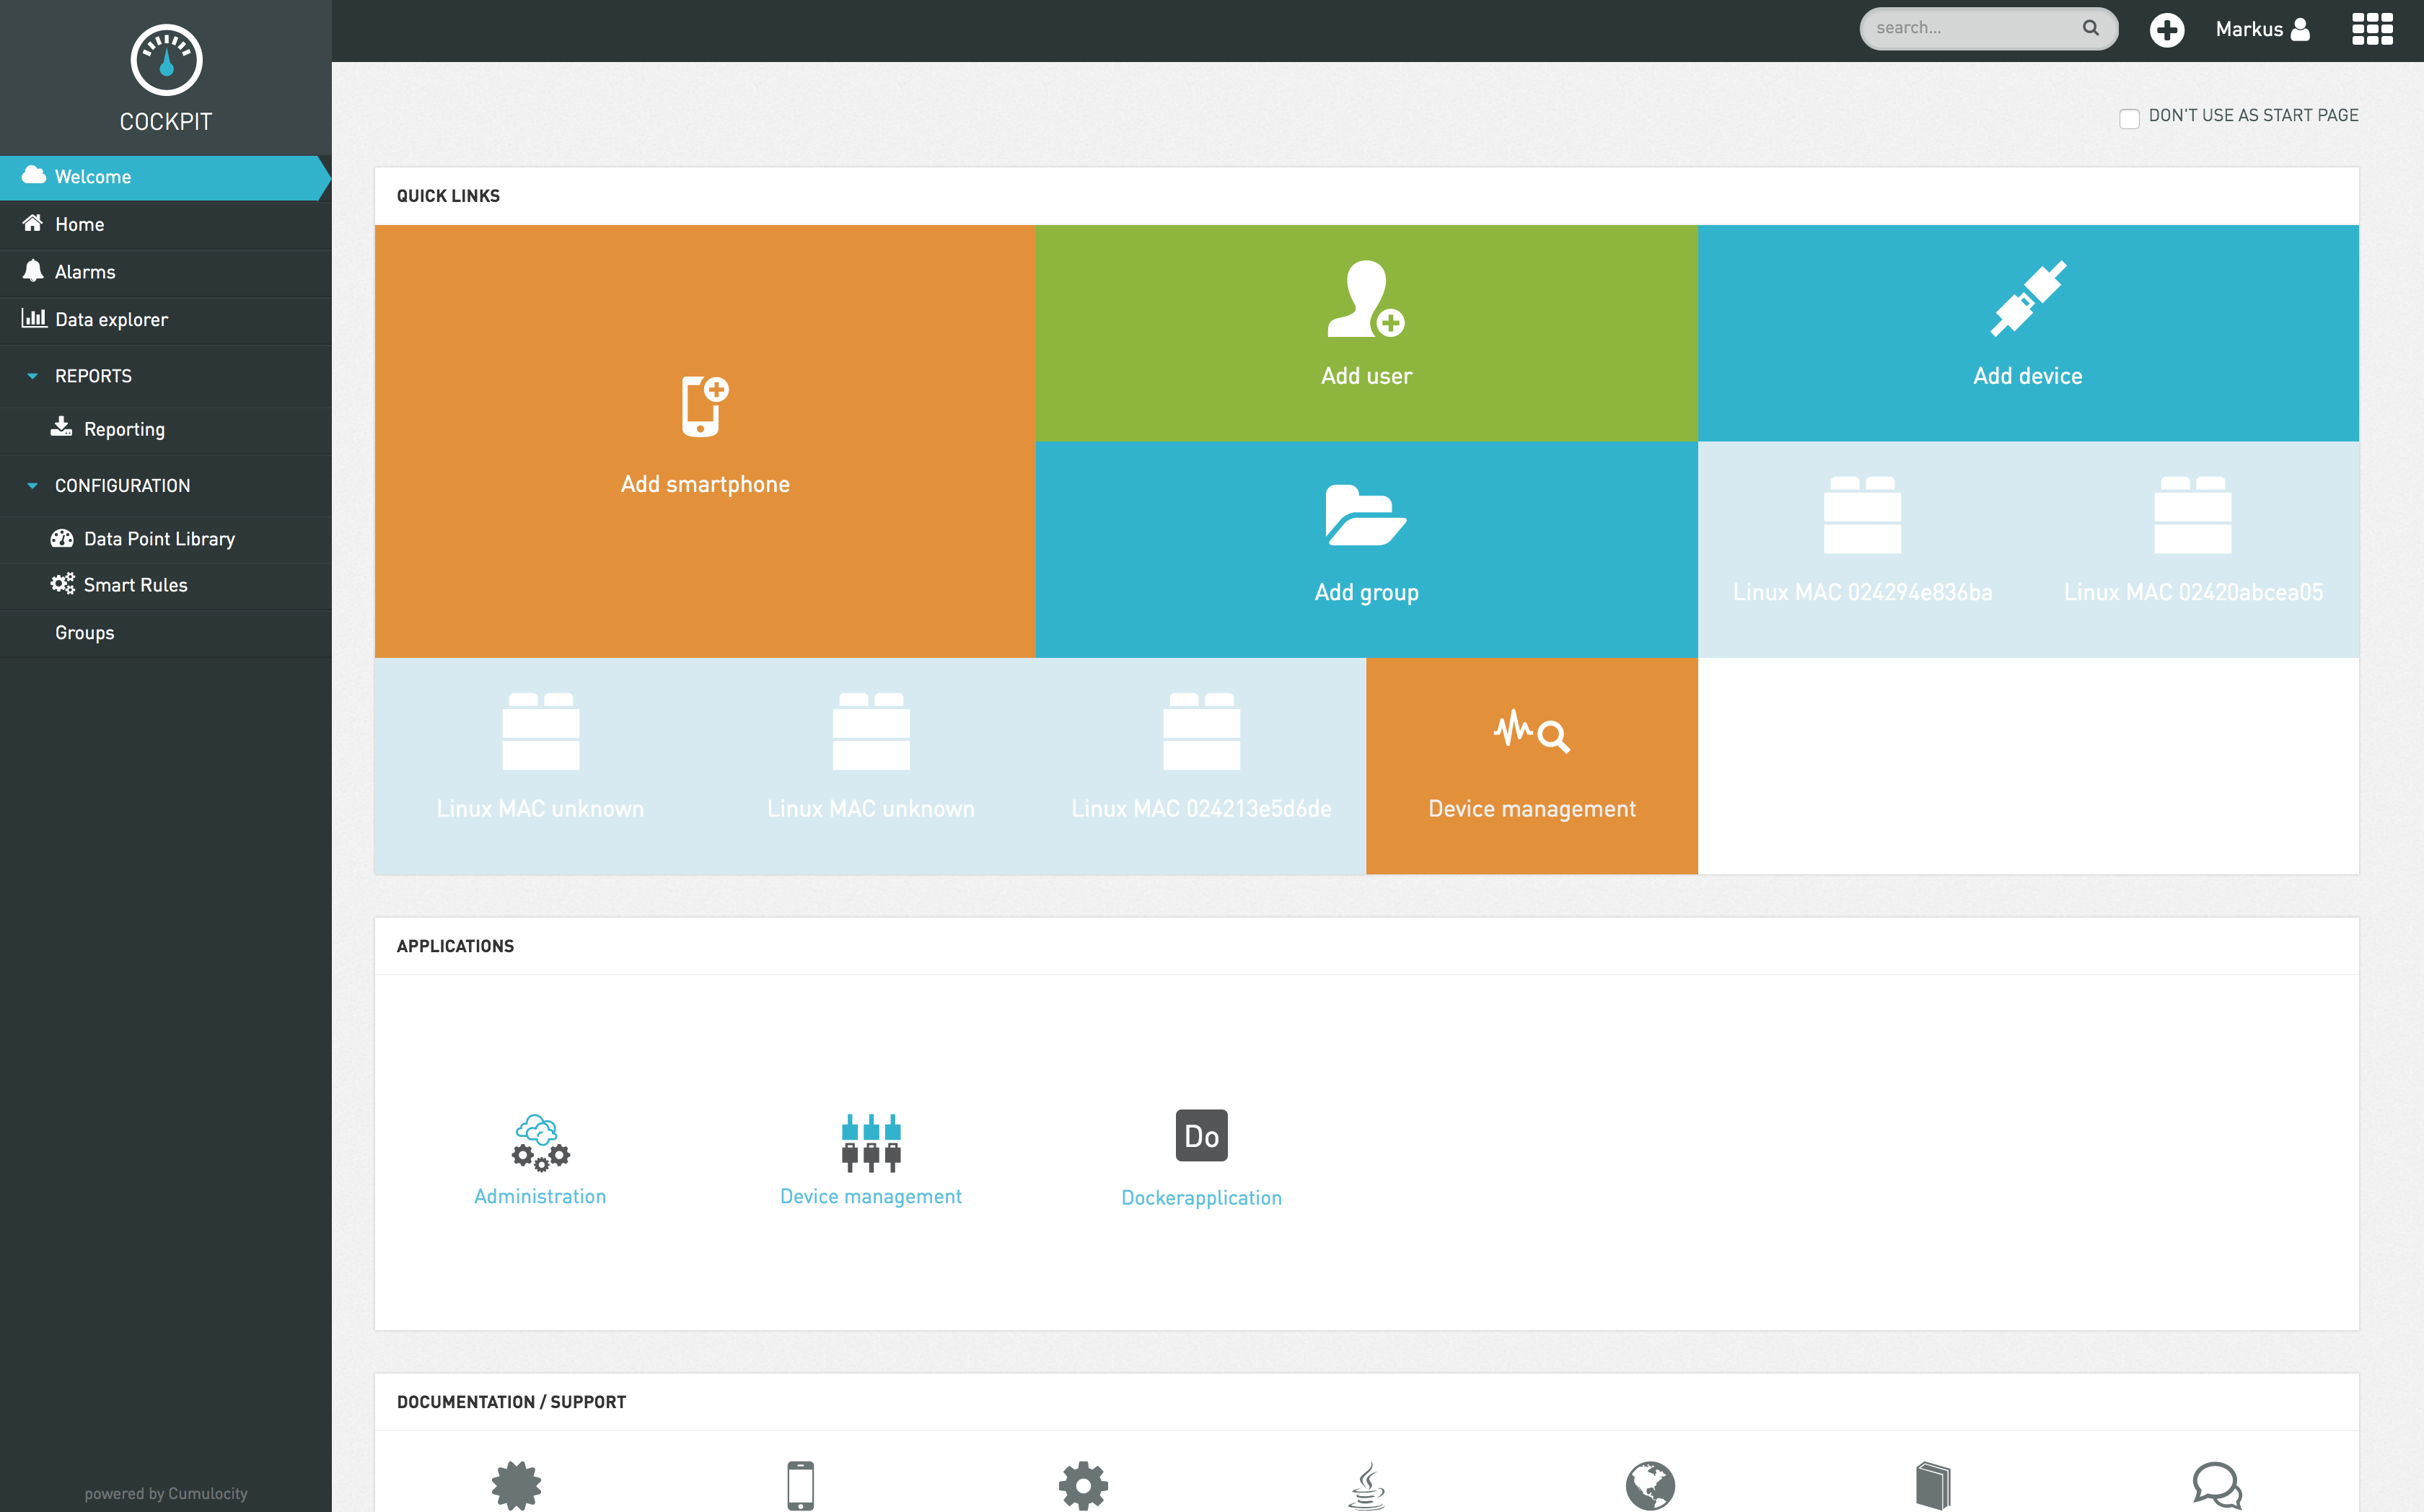
\includegraphics[width=1\textwidth]{cumulocityCockpit}
  \caption{Cumulocity kokpiti rakendus}
  \label{fig:cumulocityCockpit}
  \end{center}
  \end{figure}
  
  \FloatBarrier

  Seadmehaldus rakenduse alt on võimalik teha erinevaid toiminguid seadmetega. Nendest
  tähtsaim on seadmete registreerimine. See toimub seadmel Cumulocity agendi käivitamisega
  mille järel ilmub dialoog veebiliideses, mille alt peab seadme registreerimist kinnitama.
  Sõltuvalt agendi implementatsioonist on vahepeal vajalik enne agendi käivitamist sisestada
  seadet identifitseeriv väärtus veebiliidesesse. Iga seadme kohta on võimalik
  vaadata üldist infot; konfiguratsiooni ning identifikaatoreid
  vaadata ja muuta; seadme geograafilise asukoha lisamine, muutmine ja jälgimine;
  seadme alarme vaadata ja kustutada; seadmega seotud sündmusi vaadata. Samuti on
  reaalse seadme puudumise korral võimalik luua simuleeritud seade ning neid hallata.
  Seadmehaldus rakenduse esilehte on näha joonisel \ref{fig:cumulocityDeviceManagement}.

  \begin{figure} [ht] %try to place the figure here (next option top of the page) 
  \begin{center}
  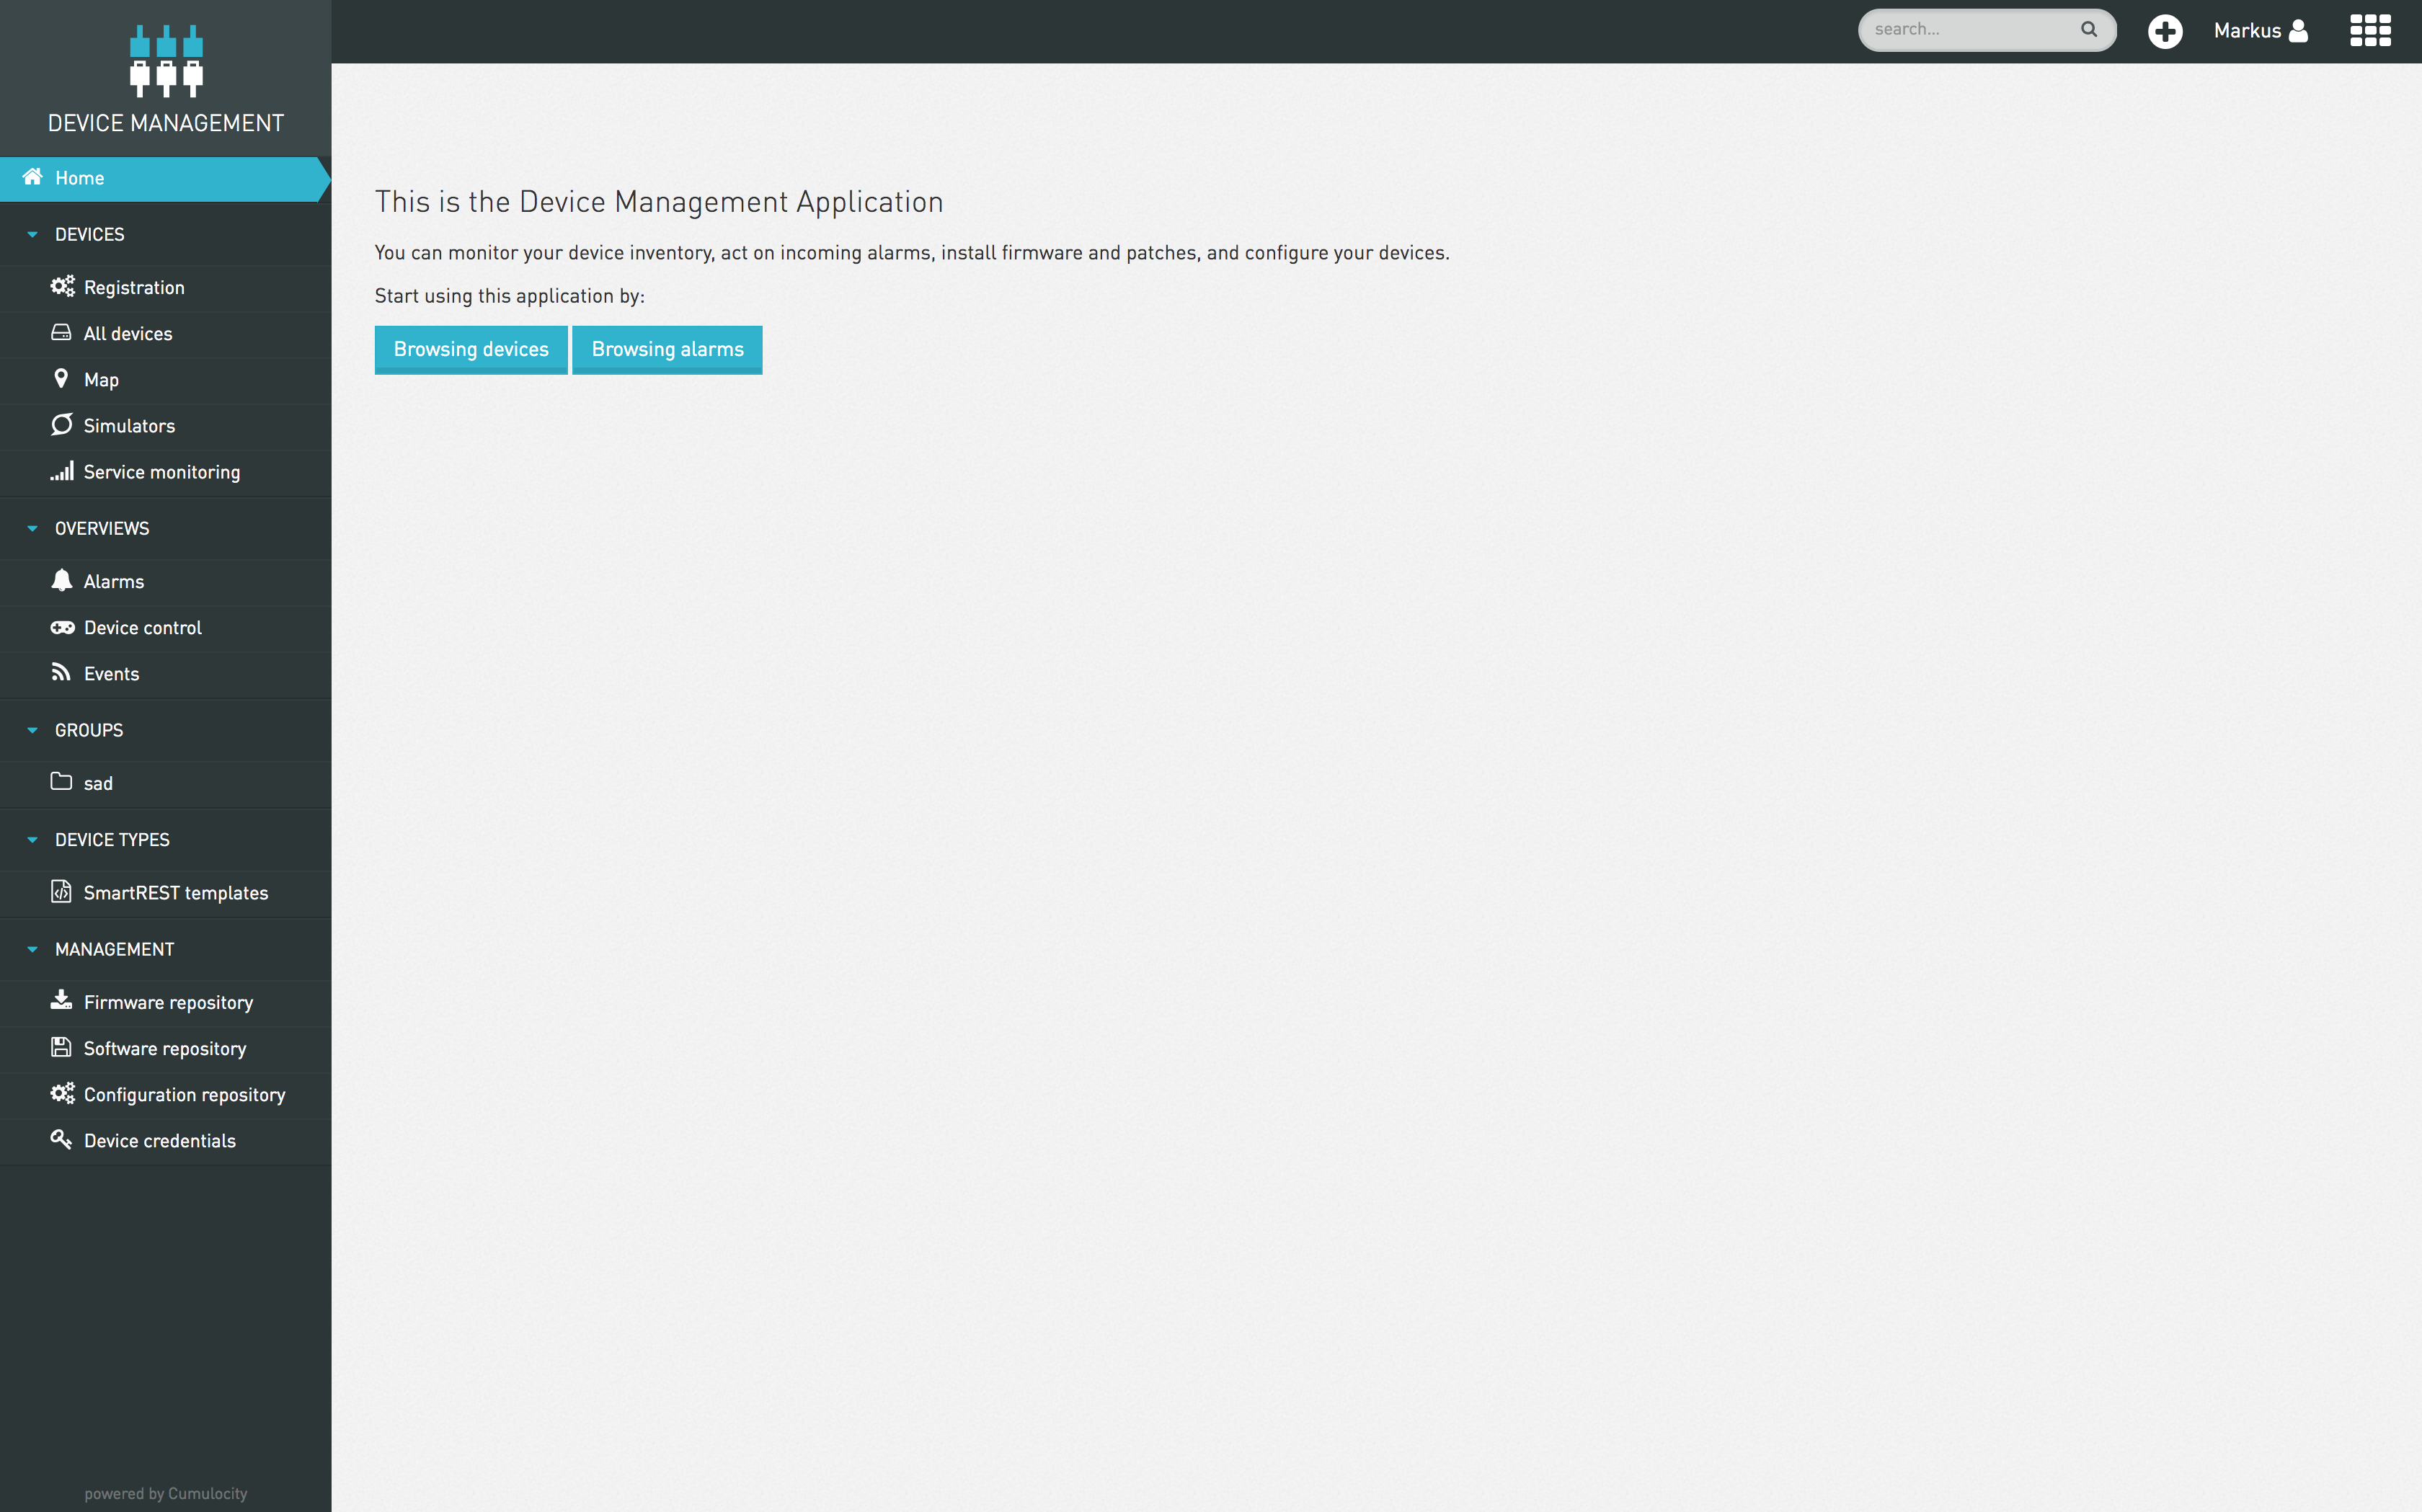
\includegraphics[width=1\textwidth]{cumulocityDeviceManagement}
  \caption{Cumulocity seadmehalduse rakendus}
  \label{fig:cumulocityDeviceManagement}
  \end{center}
  \end{figure}
  
  \FloatBarrier


  \subsection{API-liides ja seadmega suhtlus}

  Cumulocityga suhtlus käib läbi andmelao, milles hoitakse kõik seadmetega seonduv info. Andmeladu jaguneb
  mõõdistusteks, sündmusteks, alarmideks, logideks ja operatsioonideks.
  
  Mõõdistused koosnevad sensoritelt loetud
  numbrilistest andmetest näiteks temperatuuri väärtused või seadmete info põhjal arvutatud andmetest näiteks
  seadme teenuste kättesaadavus aja jooksul. Sündmusteks on kõik ülejäänud andmed, mis pärinevad sensoritelt,
  aga ei ole numbrilised väärtused näiteks ukse sensori päästmine. Sündmused võivad olla ka alarmid, kuid
  erinevalt sündmustest on alarmid prioriteetsemad ja annavad teavitusega kasutajale või süsteemi operaatorile
  teada, et kusagil esineb mingisugune viga. Alarmide teavitus püsib nii kaua, kui kasutaja või süsteemi
  süsteemi operaator märgib alarmi lahendatuks. Operatsioonid
  tähistavad andmeid, mis on saadetud seadmele käivitamiseks või töötlemiseks~\cite{CumulocityConceptsDomainModel}.
  Selleks võib olla näiteks teade elektrisaunale selle tööle panemiseks.

  Seadmetel on võimalik kasutada andmelaoga suhtlemisel Cumulocity RESTful APIt
  (inglise keeles State Transfer Application Programming Interface). See on HTTP protokollil põhinev
  programm, mis järgib REST arhitektuuri stiile. Tehes päringuid API-liidesesse saavad seadmed pärida
  infot teiste seadmete kohta ja saata andmeid platvormi. API-dega saab suhelda kindlas formaadis,
  mis sõltub API implementatsioonist~\cite{cumulocityRestDocumentation}.

  Tänapäeval on Javascripti populaarsuse tõttu tavaks kujunenud kasutada JSON formaati
  (inglise keeles JavaScript Object Notation), mis on kasutusel ka Cumulocity API-liideses.
  JSON formaat kasutab inimloetavat teksti, et edastada andmeobjekte,
  milleks on serialiseeritav väärtus näiteks sõne, number, tõeväärtus, järjend, attribuudi ja väärtuse paaridest
  koosnev objekt või nullväärtus~\cite{JSON}. 

  % RESTful API (inglise keeles Representational State Transfer Application Programming Interface) ehk rakendusliides
  % on HTTP protokollil põhinev REST arhitektuuri stiile järgiv programm, mis võimaldab teistel rakendustel integreeruda
  % teenuste või infoga tehes päringuid sellesse API-liidesesse. API-dega saab suhelda kindlas formaadis, mis sõltub API
  % implementatsioonist.
  % 
  % Tänapäeval on tavaks kujunenud kasutada JSON formaati (inglise keeles JavaScript Object Notation),
  % kuna see on tihedalt seotud JavaScriptiga ning JavaScript on olemas igas veebilehitsejas. JSON formaat
  % kasutab inimloetavat teksti, et edastada andmeobjekte, milleks on serialiseeritav väärtus näiteks 
  % sõne, number, tõeväärtus, järjend, attribuudi ja väärtuse paaridest koosnev objekt või nullväärtus.
  % Ka Cumulocity REST API-liides kasutab JSON formaati info edastamiseks.

  \begin{figure} [ht] %try to place the figure here (next option top of the page) 
  \begin{center}
  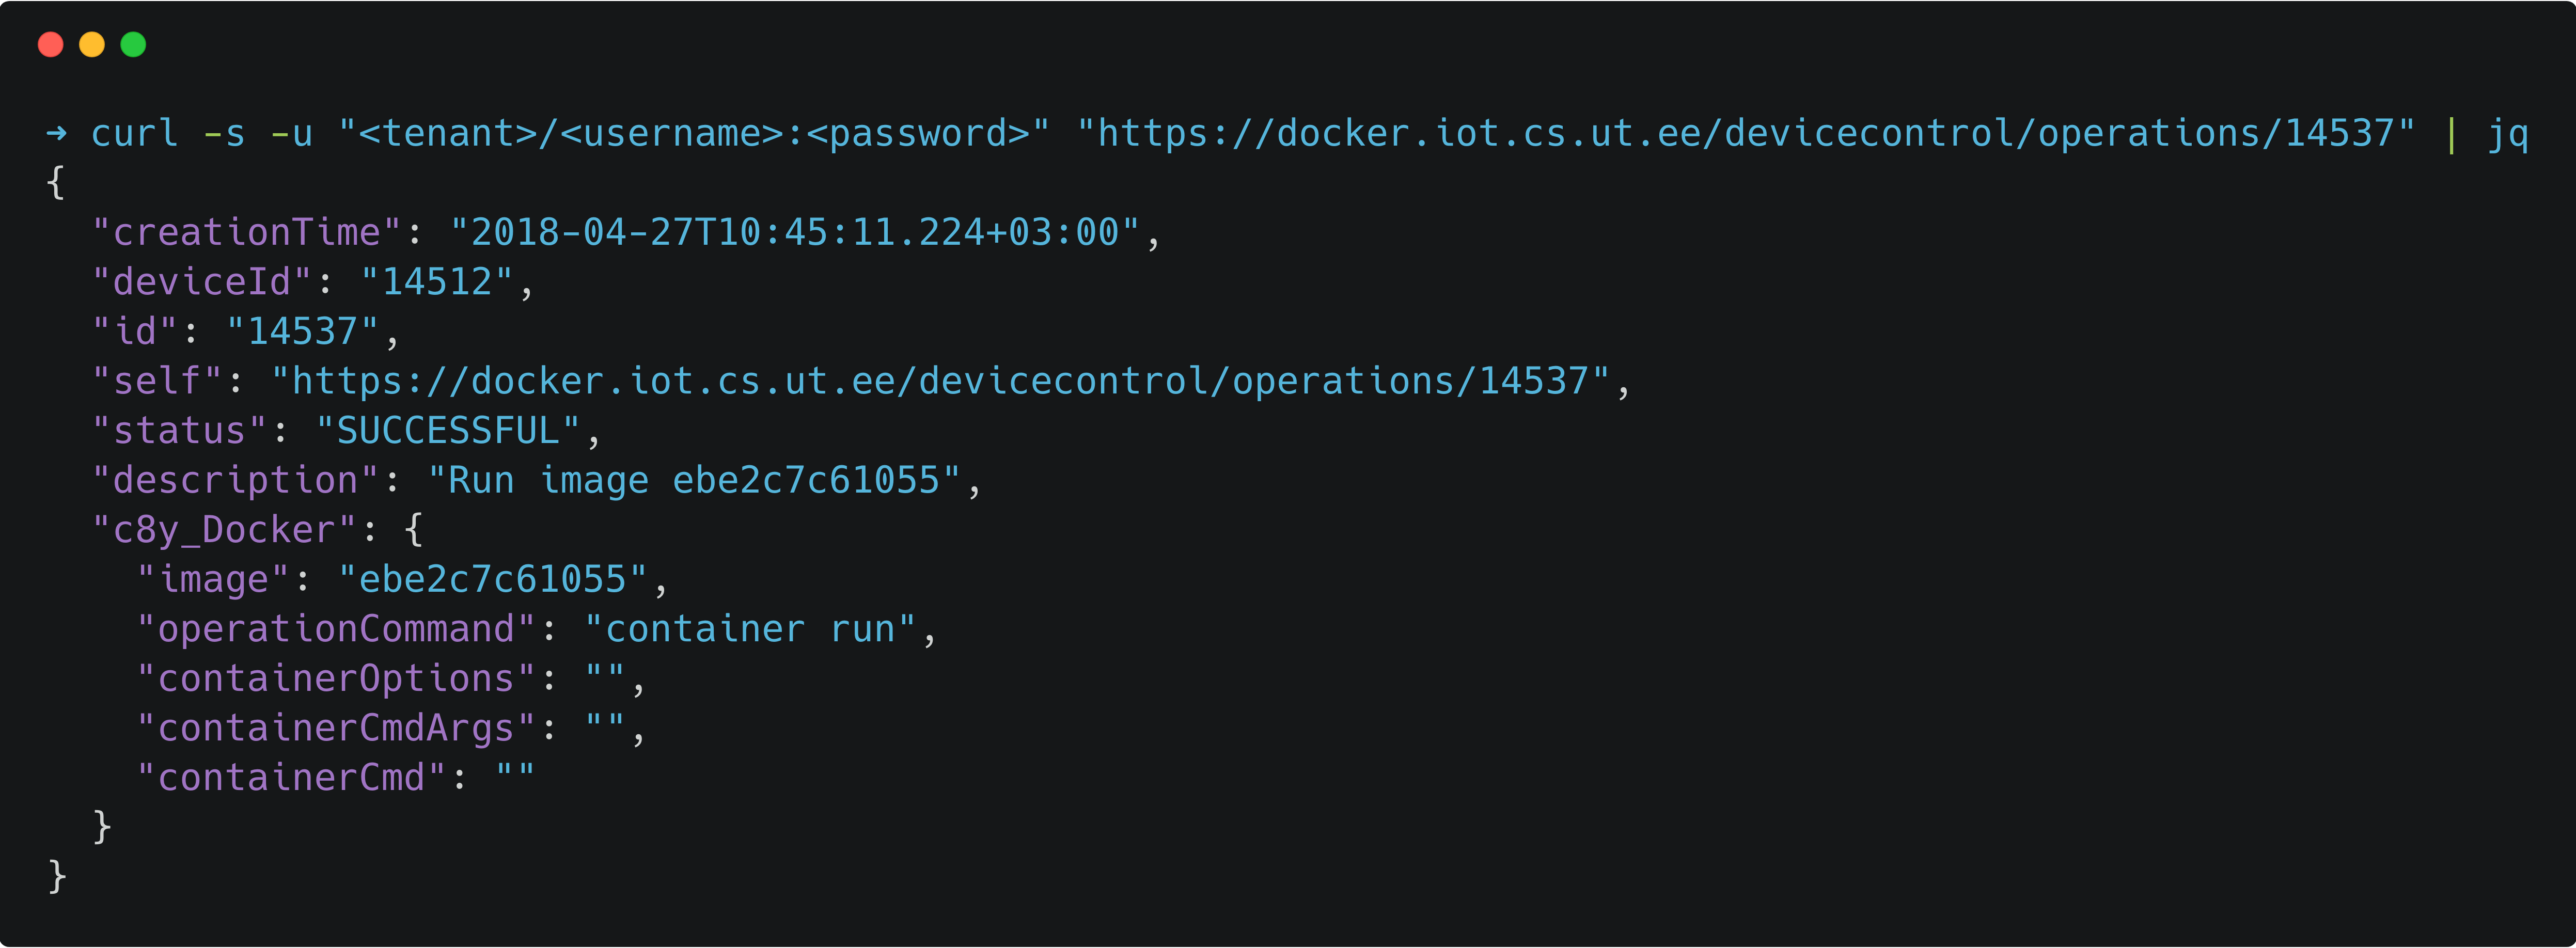
\includegraphics[width=1\textwidth]{operation14537}
  \caption{Operatsiooni andmed Cumulocity platvormis JSON formaadis}
  \label{fig:operation14537}
  \end{center}
  \end{figure}

  \FloatBarrier

  Joonisel \ref{fig:operation14537} toodud näites on tehtud curl\footnote{\url{https://curl.haxx.se/docs/manpage.html}}
  programmi abil GET päring vastu Cumulocity API-liidest.
  Päringu vastus on parema loetavuse mõttes formaaditud jq\footnote{\url{https://stedolan.github.io/jq/manual/v1.5/}}
  programmi abil, mis lisab vastusesse
  taanded ja reavahetused. Päringu tulemuseks on JSON objekt, mis sisaldab informatsiooni seadmele saadetud
  operatsiooni kohta.

  API-liides defineerib võimalikud aadressid, millele on võimalik päring teha, ja andmed, mis nendelt aadressidelt
  tagastatakse. Joonisel \ref{fig:operation14537} toodud näites aadress, mille vastu päring tehti,
  on ettemääratud Cumulocity API-liidese poolt. REST API-liides implementeerib tavaliselt 4
  päringutüüpi~\cite{REST}:

  \begin{itemize}
    \item GET - ressursist andmete pärimiseks
    \item POST - ressursis uute andmete loomiseks
    \item PUT - ressursis andmete uuendamiseks/muutmiseks
    \item DELETE - ressursis andmete kustutamiseks
    \item OPTIONS - ressursis toetatud operatsioonide pärimiseks
  \end{itemize}

  Cumulocity on teinud API-liidese võimalikult turvaliseks. API-liidese aadressid, mis peavad olema kaitstud
  kõrvaliste isikute eest, on turvatud primitiivse audentimisega (inglise keeles basic authentication). Nendele
  päringu tegemiseks on vajalik päringu päises kaasa saata kasutajanime ja parooli kombinatsioon, mis on
  omavahel ühendatud kooloniga ja kodeeritud base64 sõneks~\cite{cumulocityRestDocumentation}.
  Joonisel \ref{fig:operation14537} hoolitseb
  selle eest curl käsurea käsk, kuid allpool joonisel \ref{fig:operation14537base64} on sellest pikem näide.

  \begin{figure} [ht] %try to place the figure here (next option top of the page) 
  \begin{center}
  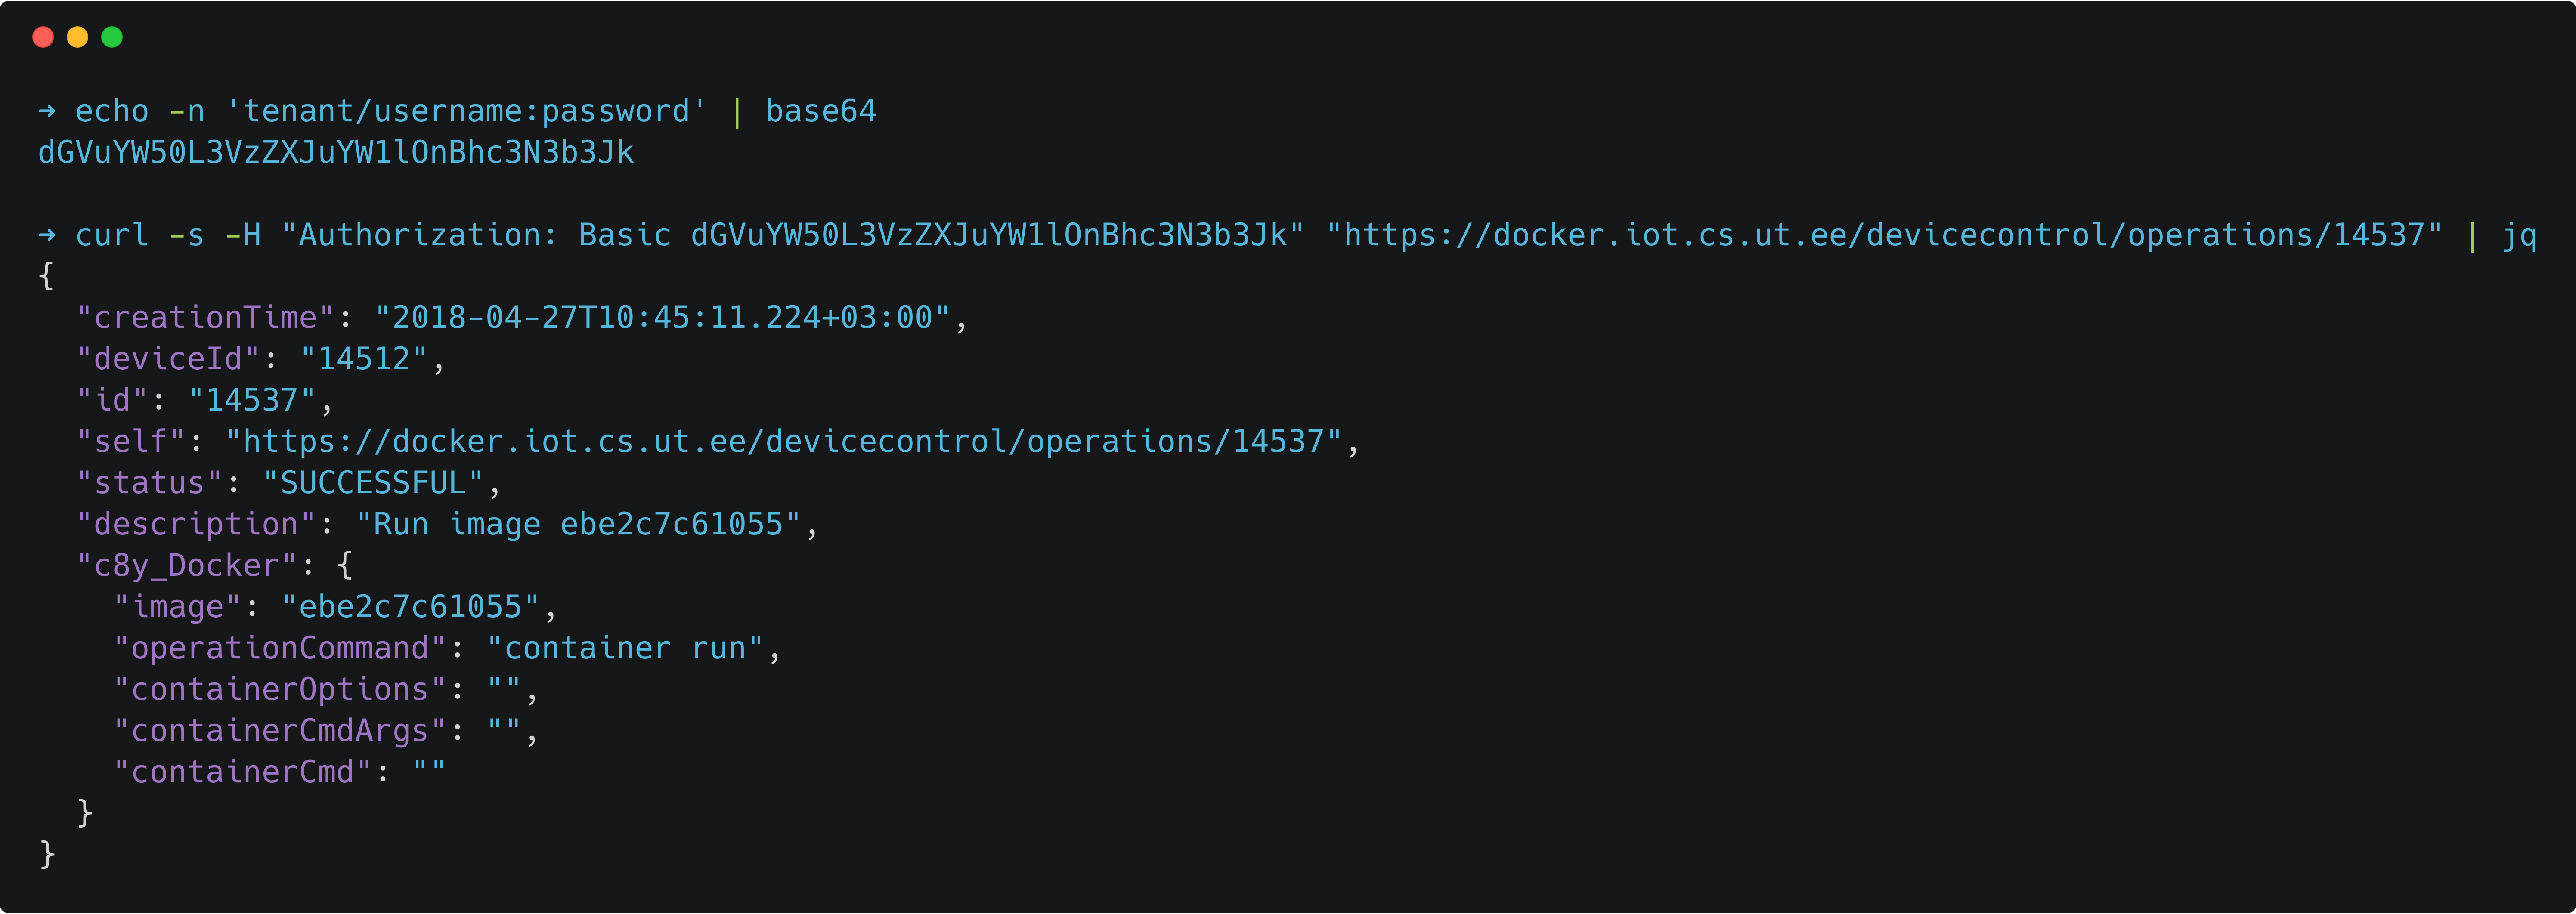
\includegraphics[width=1\textwidth]{operation14537base64}
  \caption{Operatsiooni pärimine. Audentimis päise genereerimine}
  \label{fig:operation14537base64}
  \end{center}
  \end{figure}

  \FloatBarrier

  Täpsem info Cumulocity API-liidese kohta on leitav Cumulocity veebilehel paiknevast dokumentatsioonist,
  kus kirjeldatakse võimalike aadresse, millelt saab infot pärida, ja neilt tagastatavaid
  andmeid~\cite{cumulocityRestDocumentation}.


  % REST API-liides defineerib ära võimalikud aadressid, millele on võimalik päring teha. Ülalolevas
  % näites on tehtud curl programmi abil GET päring vastu https://docker.iot.cs.ut.ee/devicecontrol/operations/13854
  % aadressi, mis on autorile kasutada antud Cumulocity tenant. REST API-liides implementeerib tavaliselt
  % 4 päringutüüpi:
  % 
  % \begin{itemize}
  %   \item GET - ressursist andmete pärimiseks
  %   \item POST - ressursis uute andmete loomiseks
  %   \item PUT - ressursis andmete uuendamiseks/muutmiskes
  %   \item DELETE - ressursis andmete kustutamiseks
  % \end{itemize}
  % 
  % Kasutades neid nelja meetodit, on võimalik läbi Cumulocity API-liiese seadmetega suhelda. 


  





  
  
  
  \newpage
  \section{Dockeri tutvustus}

  \subsection{Üldtutvustus}
  Docker on platvorm, mis pakub rakenduste arendamist ja juurutamist süsteemipiltidena
  (inglise keeles image), mis kujutavad endast väiksemahulisi iseseisvaid käivitatavaid tarkvarapakette,
  mis sisaldavad endas rakenduse koodi, käivituskeskkonda koos kõigi vajalike süsteemi
  tööriistade, rakenduse sõltuvustega ja seadistustega. Dockeri süsteemipildid on võrreldavad
  lihtsustatud operatsioonisüsteemiga. Süsteemipilte käivitades luuakse konteiner,
  milles arendaja loodud rakendus jookseb.
  \newlinespacer
  Dockeri eeliseks on lihtne rakenduse juurutamine, kuna see võimaldab jooksutada rakendust
  erinevate arvutite peal virtuaalselt samas keskkonnas. See teeb ka rakenduse arendamise
  lihtsamaks ja elimineerib arusaamatused, miks mõnes arvutis rakendus ei tööta.
  \newlinespacer
  Antud töös puutume kokku Dockeri andmetüüpidest konteinerite ja süsteemipiltidega.


  \subsection{Dockeri süsteemipildid}
  Dockeri süsteemipildid on toorikud, millest on võimalik luua toimiv süsteem. Süsteemipildi
  nimi pilt väljendub kujul ''REPOSITORY:TAG'', kus REPOSITORY on repositoorium või koodibaas,
  mida see süsteemipilt representeerib ning TAG tähistab süsteemipildi versiooni.
  Süsteemipildi loomisel tähistatakse viimane versioon ''latest'' sümboliga, kui arendaja ei ole
  teisiti määranud. Süsteemipilti saab jooksutada ''docker container run IMAGE'' käsu abil, kus IMAGE on
  süsteemipildi nimi ülaltoodud kujul. Süsteemipildi versioon ei ole kohustuslik selle käsu
  jooksutamisel - puudumisel valitakse süsteemi pildi viimane versioon ehk "latest" version.
  Käsu tulemusena luuakse Dockeri konteiner, milles süsteemipildis kirjeldatud süsteem töötab.
  
  Docker pakub võimalust hoida süsteemipilte DockerHub\footnote{https://hub.docker.com/} keskkonnas.
  Sellest on võimalik süsteemipilte alla laadida, kasutades ''docker image pull'' käsku. Süsteemipiltide
  kustutamiseks seadmelt on ''docker image rm'' käsk.

  \subsection{Dockeri konteinerid}
  Docker jooksutab protsesse isoleeritud konteinerites. Konteiner on protsess, mis jookseb
  peremeesarvutis (inglise keeles host). Peremeesarvutiks võib olla lokaalne arvuti või
  eemalasuv server. Kui kasutaja käivitab käsureal käsku ''docker container run'', siis konteineris
  on protsess isoleeritud - tal on oma failisüsteem, oma juurdepääsuvõrk ja oma
  peremeesarvutist eraldiolev isoleeritud protsessipuu. Olemasolevaid konteinereid saab
  peatada ''docker container stop'',
  taas käivitada ''docker container start'' 
  või peatada ''docker container rm'' käsu abil.



  \newpage
  \section{Praktiline osa}
  Käesolevas peatükis kirjeldatakse Cumulocity platvormi liidese loomist agendi ja veebiliidese
  mooduli näol. Kogu praktilises osas valminud kood on leitav autori Githubi
  repositooriumist (Lisa \nameref{sec:lisa_lahenduserepo}).
 
  \subsection{Nõuded}
  Loodav Cumulocity liides jaguneb kaheks: veebiliidese moodul ja agent.
  \newline
  \newline
  \noindent
  Veebiliideses seadmehaldus rakenduses seadme detailses vaates lisandub kaks vahekaarti:
  \renewcommand{\labelenumii}{\theenumii.}
  \renewcommand{\theenumii}{\theenumi.\arabic{enumii}}
  \renewcommand{\labelenumiii}{\theenumiii.}
  \renewcommand{\theenumiii}{\theenumii.\arabic{enumiii}}
  \begin{enumerate}
    \item Dockeri konteinerid
    \begin{enumerate}
      \item Kasutaja peab nägema seadmes hetkel olevaid konteinereid
      \item Kasutajal peab olema võimalik eristada töötavaid konteinereid seisvatest
     %  \item Kasutaja peab saama seisvaid konteinereid käivitada
     %  \item Kasutaja peab saama töös olevaid konteinereid peatada
     %  \item Kasutaja peab saama seisvaid konteinereid kustutada
     %  \item Kasutaja peab saama luua uusi konteinereid seadmel olemasolevatest süsteemipiltidest
      \item Kasutaja peab saama saata seadmele operatsioone seisvate konteinerite käivitamiseks
      \item Kasutaja peab saama saata seadmele operatsioone töös olevate konteinerite peatamiseks
      \item Kasutaja peab saama saata seadmele operatsioone seisvate konteinerite kustutamiseks
      \item Kasutaja peab saama saata seadmele operatsioone uute konteinerite loomiseks seadmel olevatest süsteemipiltidest
      \begin{enumerate}
        \item Konteinerite loomisel peab olema võimalus täpsustada konteineri argumente
        \item Konteinerite loomisel peab olema võimalus täpsustada konteineri sees jooksvat käsku
        \item Konteinerite loomisel peab olema võimalus täpsustada konteineri sees jooksva käsu argumente
      \end{enumerate}
  
    \end{enumerate}
    \item Dockeri süsteemipildid
    \begin{enumerate}
      \item Kasutaja peab nägema seadmes hetkel olevaid süsteemipilte
     %  \item Kasutaja peab saama seadmes süsteemipilte kustutada
     %  \item Kasutaja peab saama süsteemipilte seadmesse alla laadida
      \item Kasutaja peab saama saata seadmele operatsioone süsteemipiltide kustutamiseks
      \item Kasutaja peab saama saata seadmele operatsioone uute süsteemipiltide allalaadimiseks.
    \end{enumerate}
  \end{enumerate}
 
  \newline
  \noindent
  Cumulocity agendi nõuded
  \begin{enumerate}
    \item Agent peab oskama suhelda Dockeri käsurea programmiga
    \item Agent peab saatma Cumulocity platvormile informatsiooni Dockeri süsteemipiltide ja konteinerite kohta
    \item Agent peab oskama kuulata Cumulocity andmelattu saadetavaid operatsioone
    \item Agent peab oskama Dockeri spetsiifilise operatsioonide puhul käivitada vastavat Dockeri käsurea programmi käsku
    \item Agent peab olema lihtsasti seadmele integreeritav
    \item Kasutaja peab saama seadet platvormiga integreerida seadme identifikaatori
          sisestamisega platvormi ning seadme aksepteerimisega platvormis.
  \end{enumerate}
  
 
 %  Loodav Cumulocity liides peab võimaldama saada ülevaatliku informatsiooni seadmel töötava
 %  Dockeri oleku kohta. Cumulocity veebikeskkonnas peab olema seadme juures olema vahekaart, mille
 %  alt võimalik näha seadmel olevaid süsteemipilte, mida on võimalik juurde lisada ja kustudada.
 %  Dockeri konteinerite jaoks on teine vahekaart, mille alt on võimalik näha seadmel olevaid
 %  konteinereid, neid käivitada, peatada ja kustutada. Samuti peab saama eristada töötavaid
 %  konteinereid seistvatest. Konteinereid peab saama sama vahekaardi
 %  peal luua süsteemipiltide järgi ja peab olema võimalus lisada argumente konteineri
 %  loomise juurde. 
 
  % Loodav Cumulocity liides peab võimaldama saada ülevaatlikku informatsiooni Dockeri
  % süsteemipiltide ja konteinerite listist.
  % Agent peab olema võimeline saatma iga 5 sekundi tagant andmeid Dockeri seisu kohta.
 
  \subsection{Arhitektuur}
  Cumulocity liides koosneb kahest osast: veebiliidese moodul, mille abil saab saata seadmele
  Dockeri spetsiifilisi operatsioone, ja agent, mis oskab vastu võtta neid operatsioone.
 
  Veebiliidese moodul paikneb Cumulocity veebis ning suhtleb Cumulocity REST API-liidesega, kust
  saab infot seadmel oleva Dockeri süsteemipiltide ja konteinerite kohta ning saata
  seadmele operatsioone nende haldamiseks. Seadmel töötav agent kuulab pidevalt Cumulocity
  API-liidesest temale saadetud operatsioone ning saadab 5 sekundilise intervalli tagant
  andmeid Dockeri oleku kohta.
 
  \begin{figure} [ht] %try to place the figure here (next option top of the page) 
  \begin{center}
  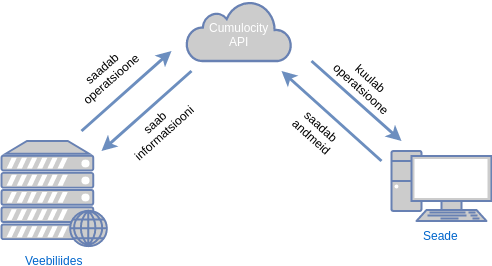
\includegraphics[width=0.6\textwidth]{architecture}
  \caption{Veebiliidese ja agendi suhtlus Cumulocity API-liidesega}
  \label{fig:architecture}
  \end{center}
  \end{figure}
 
  \FloatBarrier
 
  Veebiliidese moodul luuakse
  programmeerimiskeeles Javascript, kasutades Node.js käituskeskkonda. Node.js tuleb koos
  Npm paketihalduriga, mille abil saab installida Cumulocity liidese arendamiseks vajalikud
  sõltuvused. Esimeseks on cumulocity-tools teek, mis tagab arendusserveri ja tööriistad, mille
  abil moodul luua. Selle installimise eelduseks on Node.js versioon 6.7 või uuem.
  Teiseks on Cumulocity UI pakett, mis teeb saadavaks visuaalsed komponendid, mida
  kasutatakse hüpertekst-märgistuskeeles (HTML)
  kirjutatud mallides, mille abil mooduli kasutajaliidese kuva üles ehitatakse.
  See tagab ühtse välimuse kogu Cumulocity veebikeskkonnas.
  Teegis on olemas ka meetodid Cumulocity andmelao ja seadmetega suhtlemise jaoks.
  Kolmandaks on Lodash, mis teeb Javascripti objektidega töötamise lihtsamaks.
 
  Seadmel töötav agent luuakse Java programmeerimiskeeles. Autor otsustas agendi luua Cumulocity
  poolt valminud näitel, mis asub ettevõtte Bitbucketi repositooriumis~\cite{cumulocityExamplesRepository}.
  Näide on loodud
  väljalülitatavate moodulite põhimõttel, mis tähendab, et Dockeri funktsionaalsusega agendi
  loomiseks piisab näidisagendile uue mooduli loomisest. Autor leiab, et see tagab loodava liidese
  skaleeritavuse, kui on vaja laiendada olemasolevat agenti Dockeri funktsionaalsusega.
  % Selle jaoks on näidisagendis olemas moodul, mille abil saab olemasolevale agendile
  % lisada kompileeritud mooduli ja selle kohe kasutusele võtta.
  Agendi
  sõltuvusi haldab Maven, mis on Java projekti- ja paketihaldussüsteem.
  
  % Cumulocity poolt valminud agentide
  % näidete hulgas leidub palju kasulikke näpunäiteid.
 
  
 
 
 
  \subsection{Cumulocity veebiliidese mooduli loomine}
  % Veebiliidese loomist tuleb alustada projekti loomisega Npm abil ning sõltuvuste installimisega.
  % Selle jaoks tuleb navigeerida vabalt valitud kausta failisüsteemis, kuhu soovitakse projekt
  % salvestada ning käivitada käsureal järgmised käsud:
  % 
  % \begin{verbatim}
  % npm init --yes
  % npm install --global cumulocity-tools
  % \end{verbatim}
  % 
  % Esimene käsk loob package.json nimelise faili, mis on omane igale Node.js projektile ja
  % sisaldab endas infot projekti kohta. Teine käsk võimaldab käsureal kasutada "c8y" käsku,
  % mille abil saab teostada järgmisi operatsioone
 
  Veebiliidese moodul peab võimaldama kasutajal saada ülevaade seadmel olevate Dockeri
  konteinerite ja süsteemipiltide kohta. Süsteemipilte ja konteinereid peab saama kustutada
  ning konteinereid peab saama ka käivitada, peatada ja uusi luua.
 
  Veebiliidese mooduli loomiseks otsustati cumulocity-tools teegi poolt pakutavat arendusserverit,
  kuna see on Cumulocity poolt soovitatud viis veebiliidese mooduli arendamiseks.
  See võimaldab lokaalselt arendusmasinas testida loodavat moodulit. Seda saab käivitada
  käsurea käsuga ''c8y server -u <tenanti url>'', kus <tenanti\_url> on Cumulocity tenanti
  veebiaadress.
 
  Järgnevalt tuleb moodul konfigureerida. Dockeri süsteemipiltide ja konteinerite
  kuvamiseks on vaja luua kaks vahekaarti Cumulocity seadmehaldus lehe peale. Seda saab teha
  c8yViewsProvider abil, mis on Cumulocity UI teegist pärinev abiklass. Joonisel
  \ref{fig:webplugin_config} on näha veebiliidese mooduli konfiguratsiooni. Joonisel
  \ref{fig:webplugin_new_tabs}  on näha konfiguratsiooni tulemusena veebiliidesesse tekkivaid
  vahekaarte.
 
  \begin{figure} [ht] %try to place the figure here (next option top of the page) 
  \begin{center}
  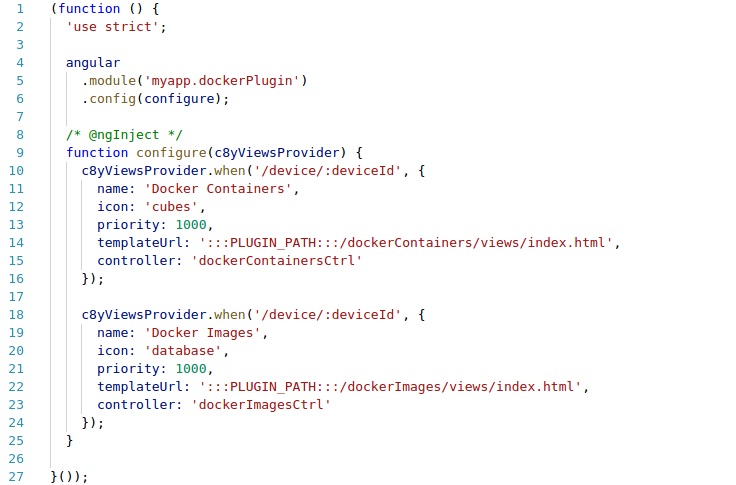
\includegraphics[width=1.0\textwidth]{webplugin_config}
  \caption{Veebiliidese mooduli konfiguratsioon}
  \label{fig:webplugin_config}
  \end{center}
  \end{figure}
  
  \FloatBarrier
 
  \begin{figure} [ht] %try to place the figure here (next option top of the page) 
  \begin{center}
  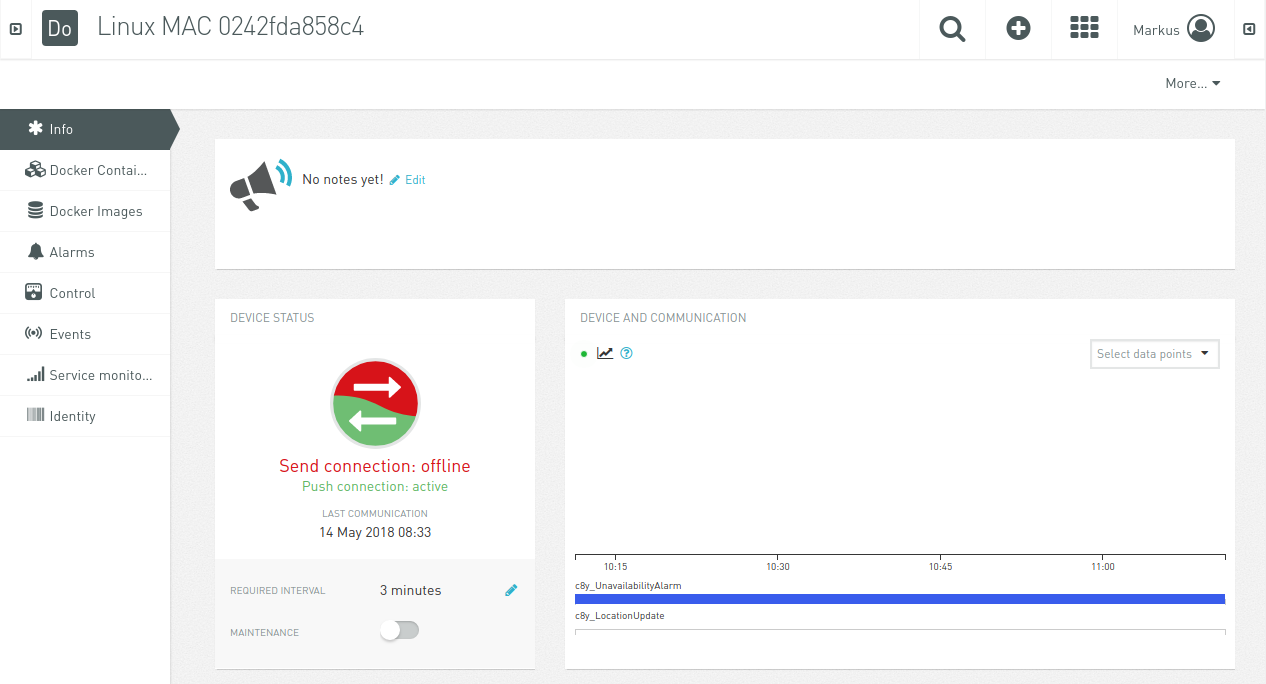
\includegraphics[width=1\textwidth]{webplugin_new_tabs}
  \caption{Uued vahekaardid Cumulocity seadmehaldus lehel. Nähtavad vasakul ääres.}
  \label{fig:webplugin_new_tabs}
  \end{center}
  \end{figure}
  
  \FloatBarrier
 
  Veebiliidese moodul peab ise hoolitsema andmete küsimise eest platvormist. Cumulocity API pihta
  päringute tegemiseks saab samuti kasutada Cumulocity UI teegis olevaid
  abiklasse\footnote{http://resources.cumulocity.com/documentation/jssdk/latest/#/api/c8y.core}.
  Seadmel oleva Dockeri oleku kätte saamiseks saab kasutada c8yDevices abiklassi,
  millega saab seadme platvormi sisese identifikaatori abil kätte seadme detailid. Nende seas
  on olemas ka informatsioon Dockeri süsteemipiltide ja konteinerite kohta.
 
  \begin{figure} [ht] %try to place the figure here (next option top of the page) 
  \begin{center}
  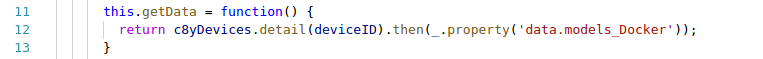
\includegraphics[width=1\textwidth]{webplugin_getimages}
  \caption{Cumulocity API-st seadme Dockeri oleku pärimine}
  \label{fig:webplugin_getimages}
  \end{center}
  \end{figure}
  
  \FloatBarrier
 
  Dockeri süsteemipiltide kuvamiseks kasutatakse hüpertekst-märgistuskeeles (HTML) kirjutatud
  malli, mida on näha joonisel \ref{fig:webplugin_images_template}. Selles on kasutatud Cumulocity UI poolt pakutavaid veebikomponente, mis tagab
  ühtse välimuse kogu ülejäänud platvormi veebiliidesega. Andmed
  kuvatakse tabeliga ''card'' komponendi sees. Samuti on malli sees olemas juba nupp süsteemipiltide kustutamise
  operatsiooni saadmiseks. Malli tulemusena genereeritud kuva on näha joonisel \ref{fig:webplugin_images}.
 
  \begin{figure} [ht] %try to place the figure here (next option top of the page) 
  \begin{center}
  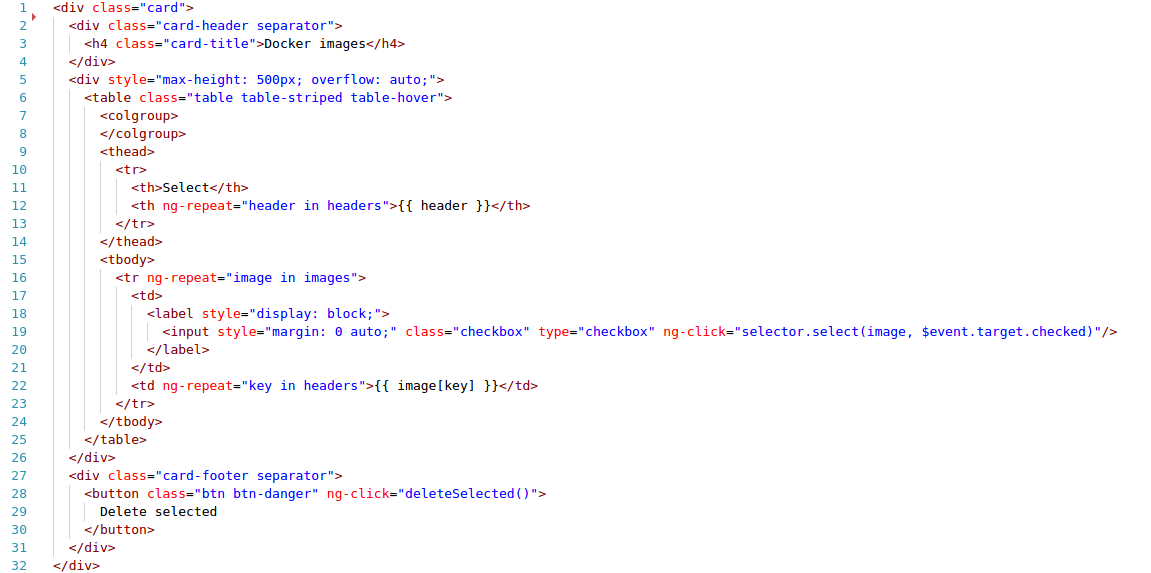
\includegraphics[width=1\textwidth]{webplugin_images_template}
  \caption{Mall süsteemipiltide kuvamiseks}
  \label{fig:webplugin_images_template}
  \end{center}
  \end{figure}
  
  \FloatBarrier
 
  \begin{figure} [ht] %try to place the figure here (next option top of the page) 
  \begin{center}
  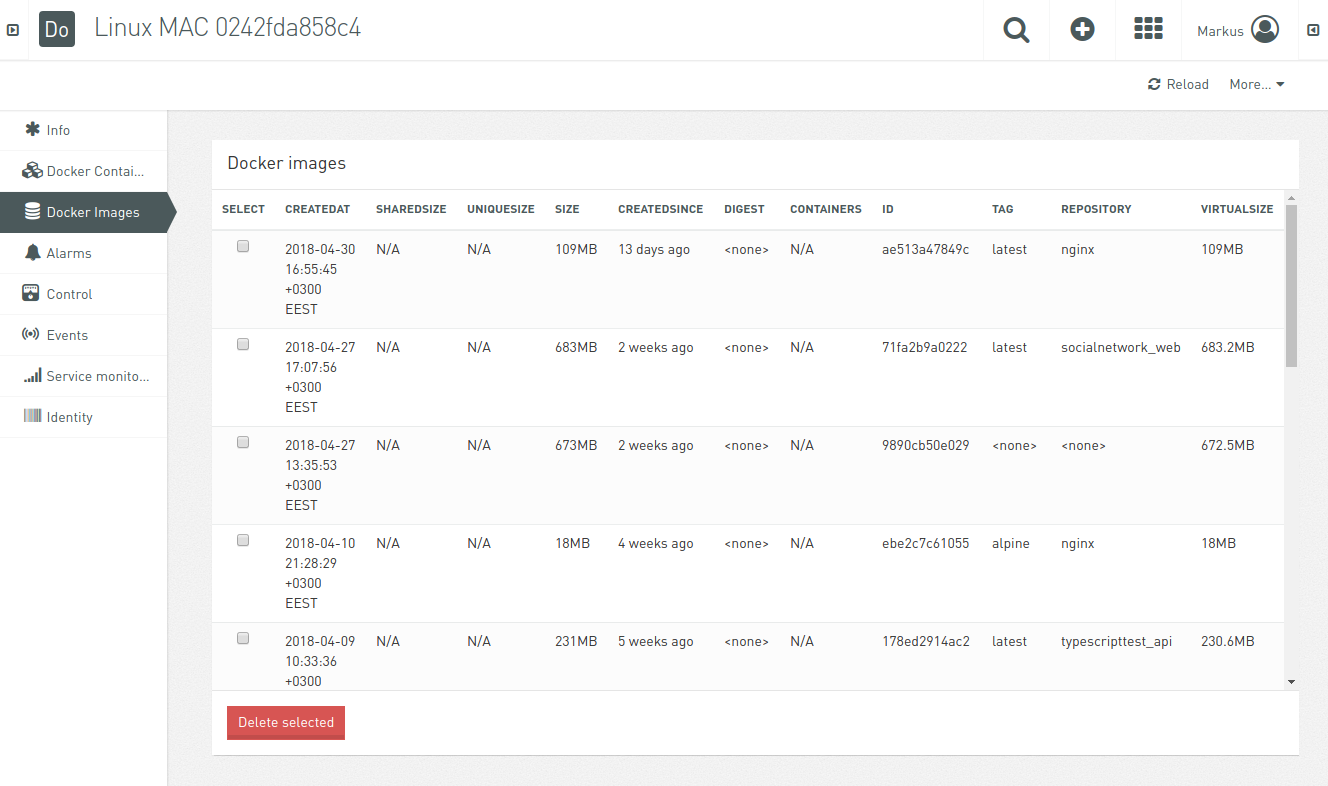
\includegraphics[width=1\textwidth]{webplugin_images}
  \caption{Süsteemipiltide kuva Cumulocity seadmehaldus lehel}
  \label{fig:webplugin_images}
  \end{center}
  \end{figure}
  
  \FloatBarrier
  
  Dockeri konteinerite kuvamise puhul on mall sarnane ja näeb välja samasugune
  nagu süsteemipiltide puhul, kuid esineb kolm nuppu
  konteinerite käivitamise, peatamise ja kustutamise operatsioonide saatmiseks. 
  Mall on nähtav joonisel \ref{fig:webplugin_containers_table_template} ja selle järgi
  genereeritud kuva joonisel \ref{fig:webplugin_containers_table}.
 
  
  \begin{figure} [ht] %try to place the figure here (next option top of the page) 
  \begin{center}
  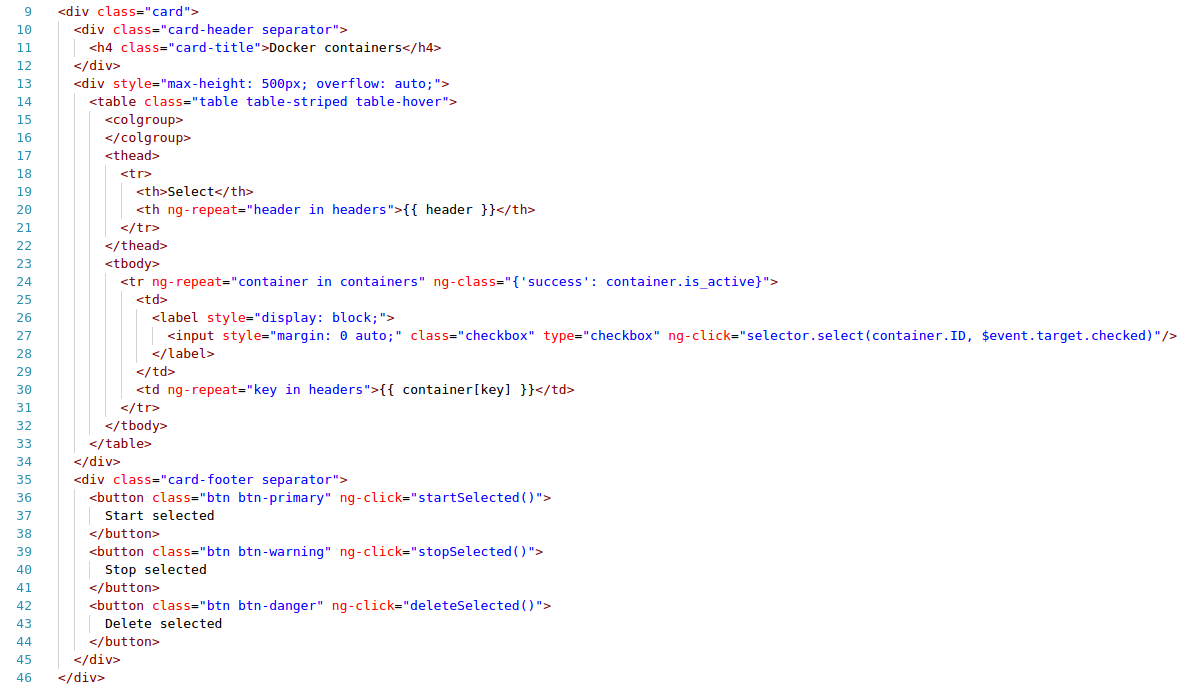
\includegraphics[width=1\textwidth]{webplugin_containers_table_template}
  \caption{Mall konteinerite kuvamiseks}
  \label{fig:webplugin_containers_table_template}
  \end{center}
  \end{figure}
  
  \FloatBarrier
 
  \begin{figure} [ht] %try to place the figure here (next option top of the page) 
  \begin{center}
  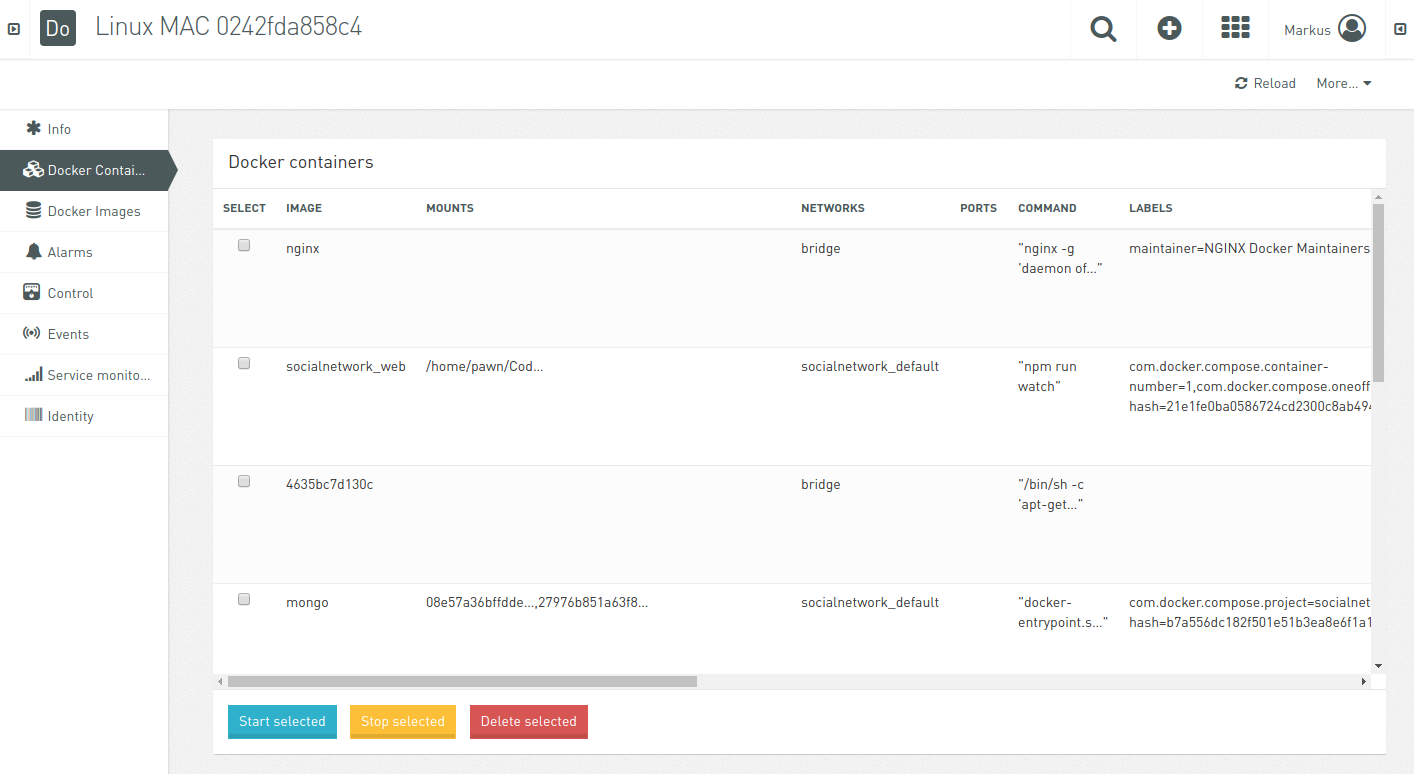
\includegraphics[width=1\textwidth]{webplugin_containers_table}
  \caption{Konteinerite kuva Cumulocity seadmehaldus lehel}
  \label{fig:webplugin_containers_table}
  \end{center}
  \end{figure}
  
  \FloatBarrier
 
  Mallis esineb ka teine ''card'' komponent. See on süsteemipiltide järgi konteinerite
  loomise operatsiooni saatmiseks, mis sisaldab endas nelja välja:
  süsteemipildi valik; konteineri käivitamise argumendid; käsk, mida jooksutatakse
  konteineri sees; argumendid konteineri sees jooksutatava käsu jaoks. Mall on
  nähtav joonisel \ref{fig:webplugin_containers_run_template} ja selle järgi 
  genereeritud kuva joonisel \ref{fig:webplugin_containers_run}.
  
  \begin{figure} [ht] %try to place the figure here (next option top of the page) 
  \begin{center}
  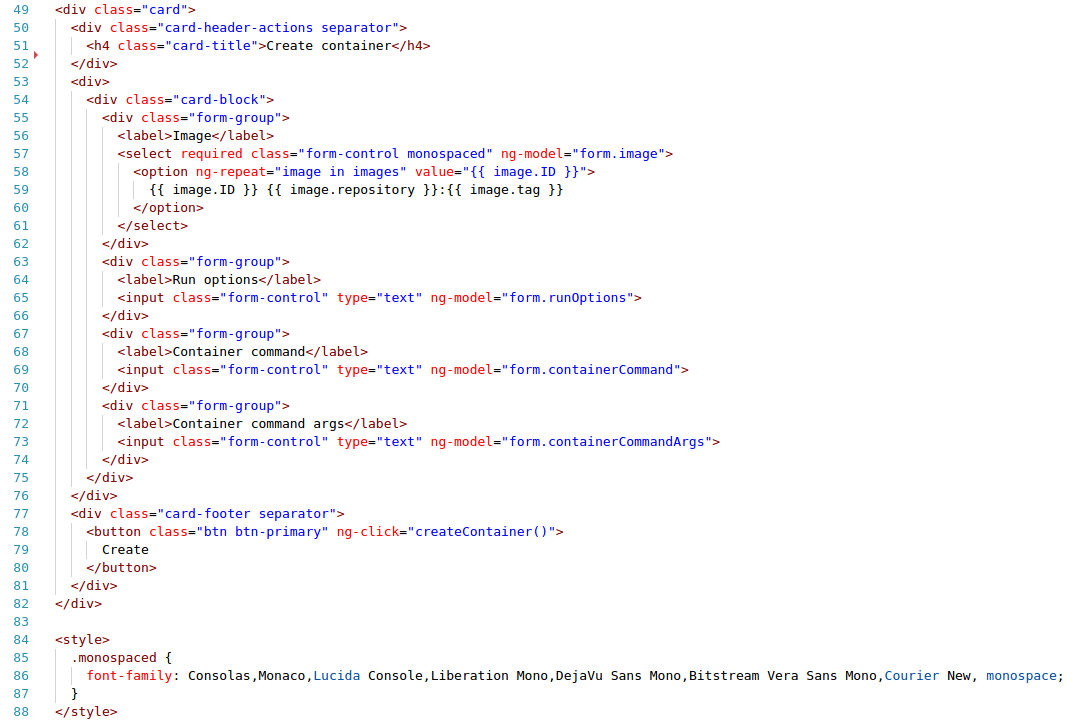
\includegraphics[width=1\textwidth]{webplugin_containers_run_template}
  \caption{Mall konteinerite käivitamiseks}
  \label{fig:webplugin_containers_run_template}
  \end{center}
  \end{figure}
  
  \FloatBarrier
 
  \begin{figure} [ht] %try to place the figure here (next option top of the page) 
  \begin{center}
  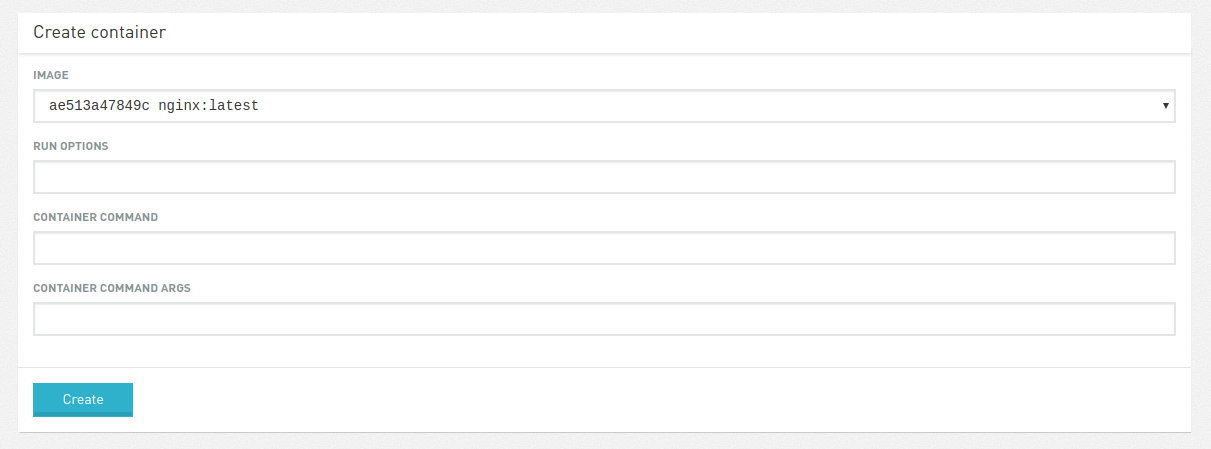
\includegraphics[width=1\textwidth]{webplugin_containers_run}
  \caption{Konteinerite loomise kuva Cumulocity seadmehaldus lehel}
  \label{fig:webplugin_containers_run}
  \end{center}
  \end{figure}
  
  \FloatBarrier
 
 
  Et mallidel olevad nupud operatsioone saadaks, on vaja luua meetodid, mis teevad päringud
  Cumulocity API-liidesesse.
  Selle kaudu operatsioonide loomiseks on Cumulocity UI teegis olemas c8yDeviceControl abiklass.
  Operatsiooni loomiseks on sellel "create", mis võtab argumendiks Javascripti objekti
  seadme identifikaatori, operatsiooni kirjeldusega ning ülejäänud osa on operatsiooni argumendid
  paaridena, kus paari esimene pool on seadme agendi poolt toetatud mooduli nimi ja paari teine
  pool on sellele moodulile saadetavad argumendid. Joonisel \ref{fig:webplugin_operationsendexample}
  on näide argumentidest.
 
  \begin{figure} [ht] %try to place the figure here (next option top of the page) 
  \begin{center}
  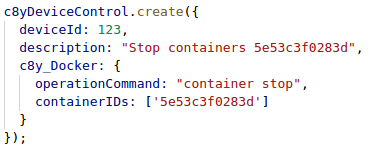
\includegraphics[width=0.6\textwidth]{webplugin_operationsendexample}
  \caption{Näide c8yDeviceControl abil operatsiooni saatmisest}
  \label{fig:webplugin_operationsendexample}
  \end{center}
  \end{figure}
  
  \FloatBarrier
 
  Autor valis agendi Dockeri mooduli nimeks ''c8y\_Docker''. Et moodul teaks,
  mida operatsiooni kätte saamisel teha, määrame moodulile saadetavate argumentide
  sisse muutuja ''dockerCommand''. Selle väärtused peavad olema veebiliidese mooduli ja
  agendi vahel kooskõlas. Kui veebist saadetakse operatsioon "container stop", siis agendi moodul
  peab teadma, mida sellise operatsiooniga teha. Seega määrame
  järgmised konstandid:
 
  \begin{itemize}
  \item image rm - Süsteemipiltide kustutamine
  \item container rm - Konteinerite kustutamine
  \item container stop - Konteinerite peatamine
  \item container start - Kontainerite käivitamine
  \item container run - Konteinerite loomine
  \end{itemize}
 
 
  Kasutades ülalmainitud konstante, luuakse joonistel
  \ref{fig:webplugin_deleteimages},
  \ref{fig:webplugin_deletecontainers},
  \ref{fig:webplugin_stopcontainers},
  \ref{fig:webplugin_startcontainers},
  \ref{fig:webplugin_createcontainer}
  näidatud meetodid, mis saadavad Cumulocity API-liidesesse operatsiooni.
  Need meetodid kutsutakse välja joonistel
  \ref{fig:webplugin_images_template},
  \ref{fig:webplugin_containers_table_template},
  \ref{fig:webplugin_containers_run_template}
  kirjeldatud nuppude vajutamisel.
 
 
  \begin{figure} [ht]
   \centering
   \begin{minipage}{0.45\textwidth}
     \centering
     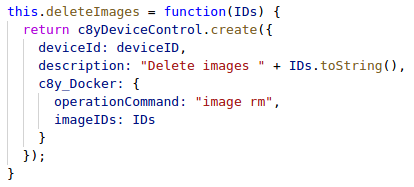
\includegraphics[width=1.0\textwidth]{webplugin_deleteimages} % first figure itself
     \caption{Meetod süsteemipiltide kustutamise operatsiooni loomiseks}
     \label{fig:webplugin_deleteimages}
   \end{minipage}\hfill
   \begin{minipage}{0.45\textwidth}
     \centering
     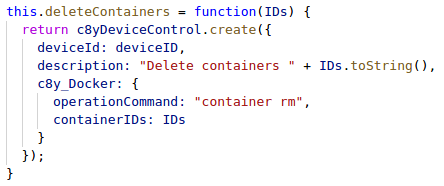
\includegraphics[width=1.0\textwidth]{webplugin_deletecontainers} % second figure itself
     \caption{Meetod konteinerite kustutamise operatsiooni loomiseks}
     \label{fig:webplugin_deletecontainers}
   \end{minipage}
  \end{figure}
 
 
  \begin{figure} [ht]
   \centering
   \begin{minipage}{0.45\textwidth}
     \centering
     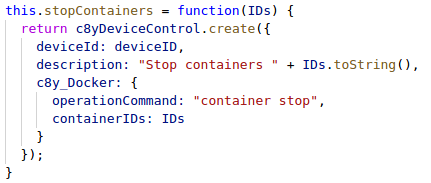
\includegraphics[width=1.0\textwidth]{webplugin_stopcontainers} % first figure itself
     \caption{Meetod konteinerite peatamise operatsiooni loomiseks}
     \label{fig:webplugin_stopcontainers}
   \end{minipage}\hfill
   \begin{minipage}{0.45\textwidth}
     \centering
     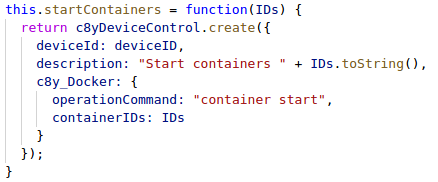
\includegraphics[width=1.0\textwidth]{webplugin_startcontainers} % second figure itself
     \caption{Meetod konteinerite käivitamise operatsiooni loomiseks}
     \label{fig:webplugin_startcontainers}
   \end{minipage}
  \end{figure}
   
  \FloatBarrier
  
  \begin{figure} [ht] %try to place the figure here (next option top of the page) 
  \begin{center}
  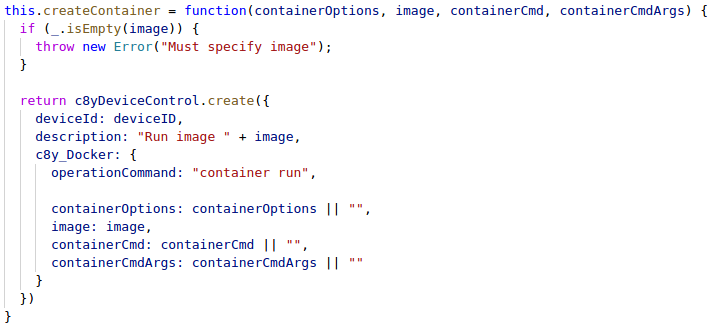
\includegraphics[width=0.8\textwidth]{webplugin_createcontainer}
  \caption{Meetod konteinerite loomise operatsiooni loomiseks}
  \label{fig:webplugin_createcontainer}
  \end{center}
  \end{figure}
  
  \FloatBarrier
 
 
   
 
 
 
  
 
 
 
 
 
 
  \subsection{Cumulocity agendi loomine}
  Agendi ülesanne on saata iga viie sekundi tagant Cumulocity andmelattu andmed
  Dockeri süsteemipiltide ja konteinerite kohta. Agent peab oskama kuulata
  operatsioonide sündmusi Cumulocity andmelaos ja seejärel vastavalt operatsioonile
  süsteemipilte või konteinereid kustutada või konteinereid käivitada, peatada, uusi luua.
 
  Loodav agent põhineb Cumulocity näidisagendi koodil, millele luuakse ''docker-driver''
  nimeline moodul Dockeri spetsiifiliste
  funktsioonide jaoks. Sellest parema arusaama saamiseks soovitab autor korra vaadata
  Cumulocity näidisagendi projekti struktuuri~\cite{cumulocityExamplesRepository}.
  Seadmel oleva Dockeriga suhtlemiseks kasutatakse Dockeri käsurea
  programmi.
  Selle välja kutsumisel peame arvestama, et see võib aega võtta ning
  seetõttu peab see olema asünkroone.
  Vastasel juhul jääb agent käsurea programmi lõpetamist ootama ning sellel ajal ei saa Cumulocity
  platvorm seadmega suhelda. Autor otsustas, et igale Dockeri spetsiifilisele Cumulocity
  operatsioonile peaks vastama klass, kus kutsutakse välja sellele operatsioonile vastav
  Dockeri käsurea programmi käsk. Selleks loodi CommandExecutor nimeline abstraktne klass,
  millest saavad operatsioonidele vastavad klassid pärineda.
 
 %  Käsurea programmide välja kutsumiseks loodi CommandExecutor nimeline
 %  klass, mida saab näha joonisel \ref{fig:dockerdriver_commandexecutor}.
 
 %  et agent ei jääks ootama käsurea programmi lõpetamist.
 %  Vastasel juhul ei ole sellel ajal võimalik platvormist seadmega suhelda,
 
 %  Selle jaoks loodi DockerRepository nimeline klass, mille abil käivitatakse Java
 %  koodi seest Dockeri käsurea programmi käsklusi. Selle jaoks on klassi sees asuv
 %  executeDockerCommand nimeline meetod. 
 
 
  \begin{figure} [ht] %try to place the figure here (next option top of the page) 
  \begin{center}
  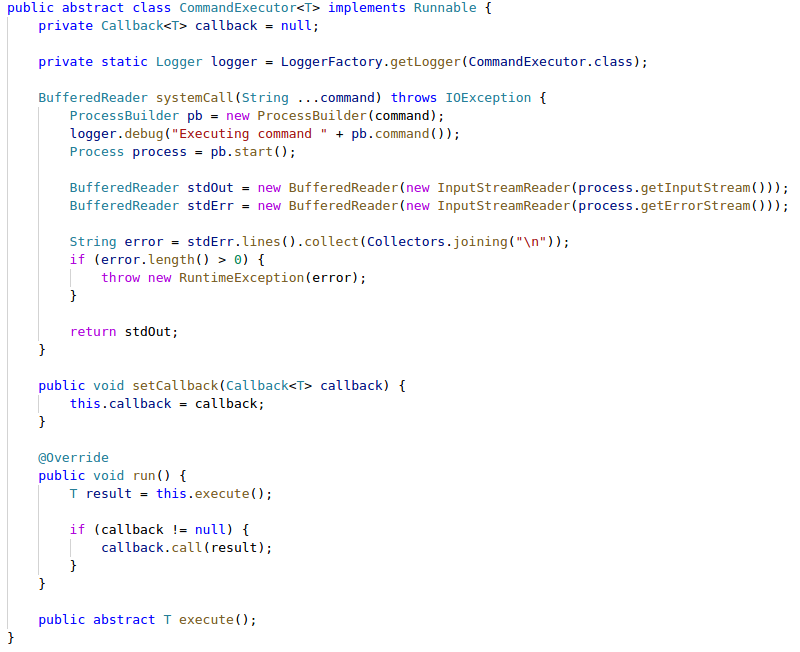
\includegraphics[width=1.0\textwidth]{dockerdriver_commandexecutor}
  \caption{CommandExecutor klass, mille abil käsurea programme käivitatakse.}
  \label{fig:dockerdriver_commandexecutor}
  \end{center}
  \end{figure}
  
  \FloatBarrier
 
 
  Joonisel \ref{fig:dockerdriver_commandexecutor} toodud CommandExecutor klass
  defineerib ''systemCall'' meetodi, mis kasutab
  käsurea programmide käivitamiseks java.lang.ProcessBuilder klassi. See võtab sisendiks
  sõnede massiivi java.lang.String[] tüüpi objektina, mille näide on järgmine:
 
  \begin{verbatim}
  # Käsurea käsk
  docker container run -p 80:80 nginx:alpine
 
  # Sama käsk ProcessBuilderis
  new String[] {"docker", "container", "run", "-p", "80:80", "nginx:alpine"}
  \end{verbatim}
 
  Autor otsustas kasutada java.lang.Thread klassi CommandExecutor klassi objektide
  asünkroonseks käivitamiseks. Seetõttu on vajalik Runnable liidese ning sellega
  kaasneva ''run'' meetodi implementeerimine. See kutsub välja ''execute'' meetodi,
  mille peavad operatsioonidele vastavad alamklassid implementeerima.
 
  Asünkroonsete tegevuste puhul ei ole teada, kuna lõppeb selle töö. Seetõttu on
  kasulik, et tegevus teavitaks mingit teist osa koodist enda lõpetamise puhul.
  Siin tuleb kasuks callback meetod, mis kutsutakse välja asünkroonse tegevuse
  lõpus. Callback meetod üldjuhul defineeritakse asünkroonse tegevuse loomisel,
  mistõttu on võimalik defineerida, mida käivitada tegevuse lõppemisel.
 
  Ka CommandExecutor klassile on võimalik defineerida callback meetod. See on
  kasulik, kui käivitada CommandExecutor klass asünkroonselt java.lang.Thread
  klassi abil. Näiteks peale Dockeri käsurea programmi lõppemist saab callback
  meetodi sees saata Cumulocity platvormi uue informatsiooni Dockeri
  süsteemipiltide ja konteinerite kohta.
  Aga autor jättis võimaluse kutsuda CommandExecutor klassi
  ka sünkroonselt välja juhul kui on vaja koheselt tulemust teada saada.
  Sellisel juhul ei ole callback meetod vajalik. Et määrata
  callback meetodi tüüpi, loodi Callback nimeline liides, mis on nähtav
  jooniselt \ref{fig:dockerdriver_callback}.
 
  % Peale Dockeri käsurea programmi
  % lõppemist on vajalik saata Cumulocity platvormi uus informatsioon Dockeri seisu
  % kohta. Seetõttu on vaja callback meetodit, mida kutsuda välja ''run'' meetodi
  % lõpus, et saata tulemus tagasi CommandExecutor alamklassi väljakutse juurde.
  % Selleks defineeriti Callback nimeline liides, mis väljendab callback meetodi
  % tüüpi. See on nähtav jooniselt \ref{fig:dockerdriver_callback}.
 
  \begin{figure} [ht] %try to place the figure here (next option top of the page) 
  \begin{center}
  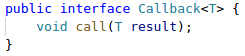
\includegraphics[width=0.4\textwidth]{dockerdriver_callback}
  \caption{Callback liides, mis määrab callback meetodi tüübi.}
  \label{fig:dockerdriver_callback}
  \end{center}
  \end{figure}
  
  \FloatBarrier
 
  % Callback meetod on vajalik ainult CommandExecutor klassi asünkroonse välja kutsumise
  % korral, kuna asünkroonse käivituse korral ei ole teada, kuna 
 
 
  % Käsurea käskude asünkroonseks väljakutsumiseks on kasulik kasutada java.lang.Thread
 
 
  % implementeerib Runnable liidest. See võimaldab kutsuda klassi sees olevat koodi
  % java.lang.Thread klassi abil asünkroonselt välja, mis on kasulik kaua aega
  % võtvate käsurea programmide käivitamisel.
  % Runnable liides nõuab ''run'' meetodi defineerimist, 
 
  % Selle abil saab CommandExecutor alamklasse kutsuda
  % välja ka asünkroonselt kasutades java.lang.Thread klassi. See on kasulik Dockeri spetsiifiliste
  % Cumulocity operatsioonide käivitamiseks, kuna neid saab käivitada nii, et 
  
  % kasutatakse
 
  
  
  % mis sisaldab endas käsku ja selle argumente tokeniseeritud kujul ning
  % tekitab käsust protsessi ja annab argumendid otse 
 
  Kasutades joonisel \ref{fig:dockerdriver_commandexecutor} näidatud CommandExecutor klassi,
  luuakse Dockeri spetsiifilistele Cumulocity operatsioonidele klassid, mis pärinevad
  CommandExecutor klassid. Kuna need erinevad põhiliselt ainult Dockeri käsurea programmi
  käsu poolest, siis autor toob välja ainult Dockeri süsteemipiltide kustutamiseks ja Dockeri
  konteinerite loomiseks loodud klassid, mis on nähtavad
  joonistel \ref{fig:dockerdriver_dockerimagermcommand} ja \ref{fig:dockerdriver_dockercontainerruncommand}.
 
 
  \begin{figure} [ht] %try to place the figure here (next option top of the page) 
  \begin{center}
  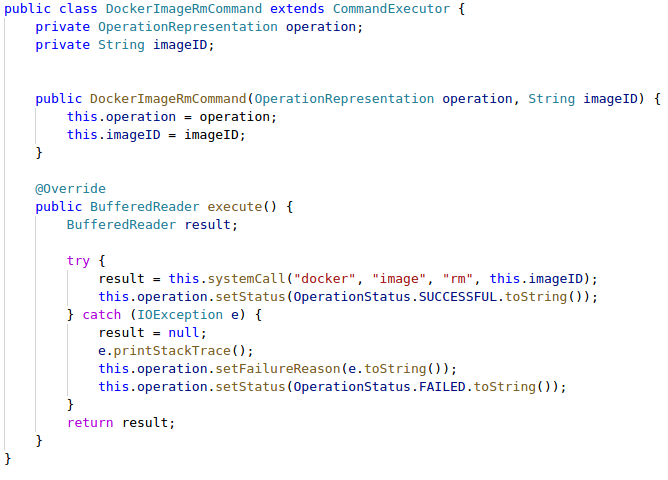
\includegraphics[width=1.0\textwidth]{dockerdriver_dockerimagermcommand}
  \caption{Klass DockerImageRmCommand, mis võimaldab Dockeri süsteemipilte kustutada}
  \label{fig:dockerdriver_dockerimagermcommand}
  \end{center}
  \end{figure}
  
  \FloatBarrier
 
 
  \begin{figure} [ht] %try to place the figure here (next option top of the page) 
  \begin{center}
  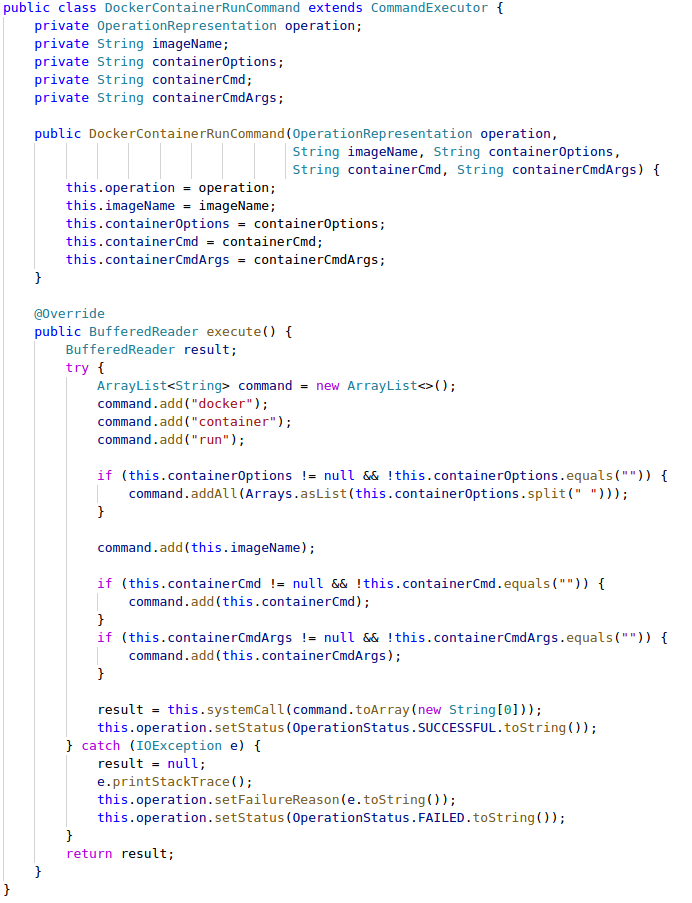
\includegraphics[width=1.0\textwidth]{dockerdriver_dockercontainerruncommand}
  \caption{Klass DockerContainerRunCommand, mis võimaldab Dockeri konteinereid luua}
  \label{fig:dockerdriver_dockercontainerruncommand}
  \end{center}
  \end{figure}
  
  \FloatBarrier
 
 
  Agendi operatsioonide kuulamine on juba Cumulocity näidisagendis ette defineeritud.
  Agent kuulab operatsioonide sündmusi andmelaos, mis sinna läbi API-liidesesse
  saadetakse, ja operatsiooni
  saabumisel saadetakse see agendi moodulitele laiali. Moodul peab seejärel aru
  saama, kas operatsioon oli talle suunatud või mõnele muule moodulile. Kuna
  agent kuulab kõiki operatsioone andmelaos, siis peab moodul otsustama ka,
  kas operatsioon on mõeldud sellele seadmele või mitte.
 
  Loodava agendi mooduli keskmeks on DockerDriver nimeline klass, mis suhtleb Cumulocity platvormiga.
  Selleks, et agent teaks, et moodul toetab operatsioonide käivitamist, peab
  DockerDriver klass implementeerima c8y.lx.driver.OperationExecutor
  liidese, mis nõuab, et moodul teataks oma operatsiooni tüübi,
  milleks on ''c8y\_Docker'' nagu joonise
  \ref{fig:webplugin_operationsendexample} juures kirjeldatud on. Selleks peab
  defineerima joonisel \ref{fig:dockerdriver_supportedoperationtype} kirjeldatud
  kaks meetodit.
 
  \begin{figure} [ht] %try to place the figure here (next option top of the page) 
  \begin{center}
  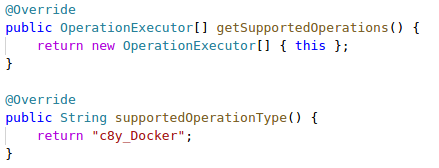
\includegraphics[width=0.6\textwidth]{dockerdriver_supportedoperationtype}
  \caption{Meetodid Dockerdriver klassis, mis teatavad toetatud operatsiooni tüübi agendile}
  \label{fig:dockerdriver_supportedoperationtype}
  \end{center}
  \end{figure}
  
  \FloatBarrier
  
  OperationExecutor liides ka nõuab ''execute'' meetodi defineerimist. Selles meetodis peab
  kontrollima, kas operatsioon on mõeldud sellele seadmele. Veebiliideses saadetud
  Dockeri operatsioonid sisaldavad endas ''dockerCommand'' muutujat nagu joonise
  \ref{fig:webplugin_operationsendexample} juures kirjeldatud on. Selle järgi saab ''execute''
  meetodis teada, millist Dockeri käsurea käsku jooksutada. 
 
  \begin{figure} [ht] %try to place the figure here (next option top of the page) 
  \begin{center}
  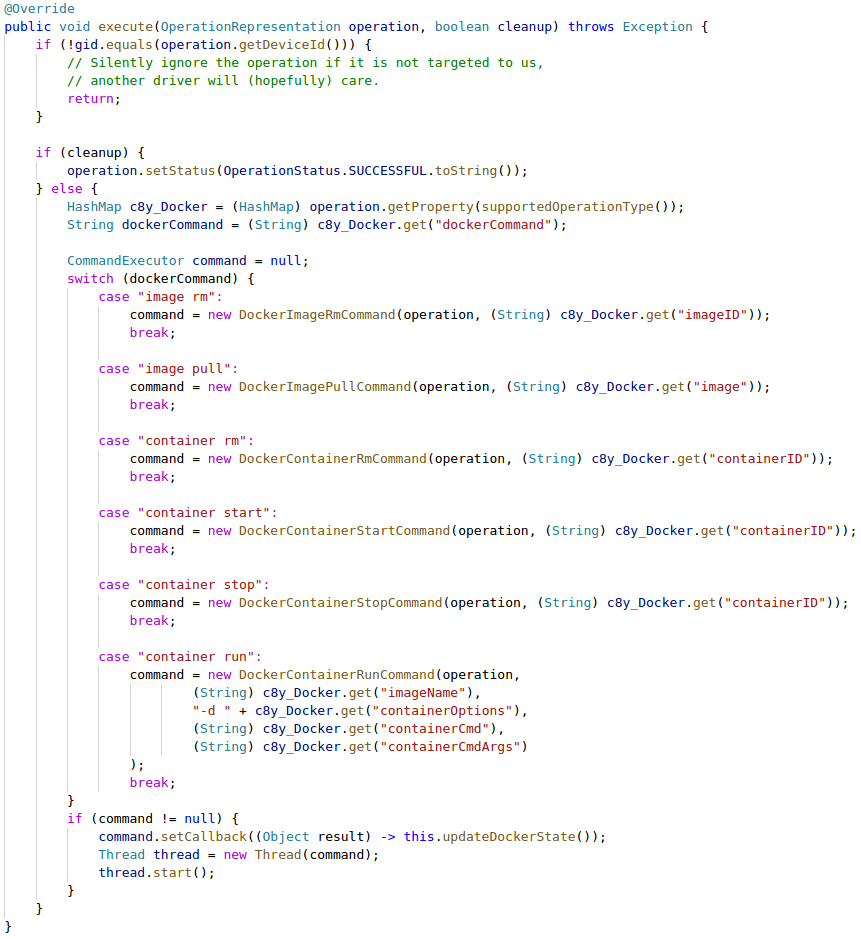
\includegraphics[width=1.0\textwidth]{dockerdriver_execute}
  \caption{Meetod execute DockerDriver klassis, mis käivitab vastava Dockeri käsurea programmi sõltuvalt operatsioonist}
  \label{fig:dockerdriver_execute}
  \end{center}
  \end{figure}
 
  \FloatBarrier
 
 
  Nüüdseks oskab DockerDriver klass võtta vastu veebiliidese moodulist saadetavaid
  Dockeri operatsioone. Selleks, et see oskaks saata informatsiooni Dockeri konteinerite
  ja süsteemipiltide kohta peab DockerDriverit laiendama. Selleks on c8y.lx.driver
  paketis olemas PollingDriver nimeline klass. See implementeerib java.lang.Runnable
  liidest, mistõttu on vaja DockerDriver klassis defineerida ''run'' meetod.
  PollingDriver kutsub seda meetodit ajalise intervalli tagant välja, milleks on
  DockerDriver klassis määratud 5 sekundit. Selle meetodi sisse saab implementeerida
  platvormi informatsiooni saatmise, aga enne on vaja defineerida mudelid, milles hoida
  informatsiooni Dockeri konteinerite ja süsteemipiltide kohta. Nendeks on tavalised
  klassid, mis koos oma väljadega on informatsiooni esitusviisiks. Need on nähtavad
  joonistel \ref{fig:dockerdriver_dockercontainer} ja \ref{fig:dockerdriver_dockerimage}.
 
  \begin{figure} [ht] %try to place the figure here (next option top of the page) 
  \begin{center}
  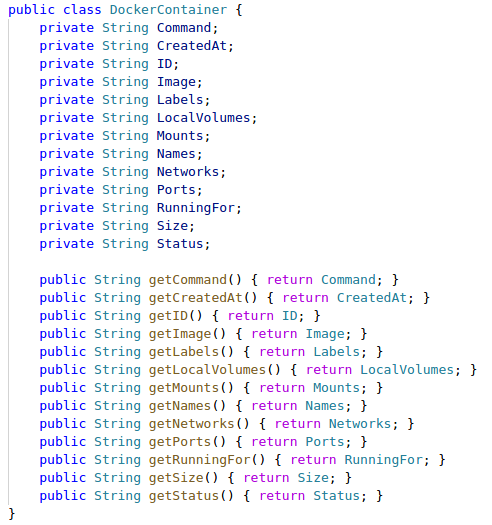
\includegraphics[width=0.6\textwidth]{dockerdriver_dockercontainer}
  \caption{Klass DockerContainer süsteemipiltide hoidmiseks}
  \label{fig:dockerdriver_dockercontainer}
  \end{center}
  \end{figure}
 
  \FloatBarrier
  
 
  \begin{figure} [ht] %try to place the figure here (next option top of the page) 
  \begin{center}
  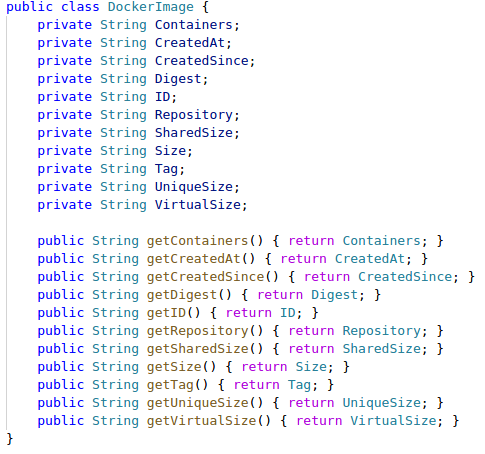
\includegraphics[width=0.6\textwidth]{dockerdriver_dockerimage}
  \caption{Klass DockerImage süsteemipiltide hoidmiseks}
  \label{fig:dockerdriver_dockerimage}
  \end{center}
  \end{figure}
 
  \FloatBarrier
 
 
  Informatsiooni Dockeri konteinerite ja süsteemipiltide kohta saab Dockeri käsurea programmist.
  See kuvab tavaliselt andmed tabelina, kus näiteks süsteemipiltide puhul kuvab üks rida ühe
  süsteemipildi andmed. Õnneks on Dockeri käsurea programmil olemas
  \verb|--format '{{ json . }}'| lipp, mis kuvab andmeid JSON formaadis, kuid väljundiks
  on JSON objekti asemel read, kus üks rida on üks JSON objekt, mis tähistab ühte süsteemipilti.
  Seda on kerge parsida
  mudelitesse, milleks autor kasutas com.google.gson\footnote{https://github.com/google/gson}
  teegist GSON klassi, kuna autor on sellega varasemalt kokku puutunud. Kuna Dockeri käsurea
  programmi väljundis on üks rida üks JSON objekt, siis tuleb parsida terve väljundi asemel
  igat rida eraldi. Dockeri käsurea programmi väljundi parsimist demonstreerib joonis
  \ref{fig:dockerdriver_jsonparse}.
  
 
  \begin{figure} [ht] %try to place the figure here (next option top of the page) 
  \begin{center}
  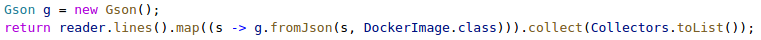
\includegraphics[width=1.0\textwidth]{dockerdriver_jsonparse}
  \caption{Dockeri käsurea programmi väljundi parsimine DockerImage mudeliteks. Muutuja ''reader'' on klassi BufferedReader objekt.}
  \label{fig:dockerdriver_jsonparse}
  \end{center}
  \end{figure}
 
  \FloatBarrier
 
 
  Seadmel olevate Dockeri süsteemipiltide ja konteinerite kättesaamiseks loodi joonisel
  \ref{fig:dockerdriver_commandexecutor} olevast CommandExecutor klassist joonistel
  \ref{fig:dockerdriver_dockerimagelscommand} ja \ref{fig:dockerdriver_dockerimagelscommand}
  klassid. Mõlemad käivitavad Dockeri käsurea programmi, mis tagastab kummalegi andmed
  süsteemipiltide ja konteinerite kohta ning seejärel parsitakse need andmed joonisel
  \ref{fig:dockerdriver_jsonparse} näidatud viisil mudeliteks.
 
  \begin{figure} [ht] %try to place the figure here (next option top of the page) 
  \begin{center}
  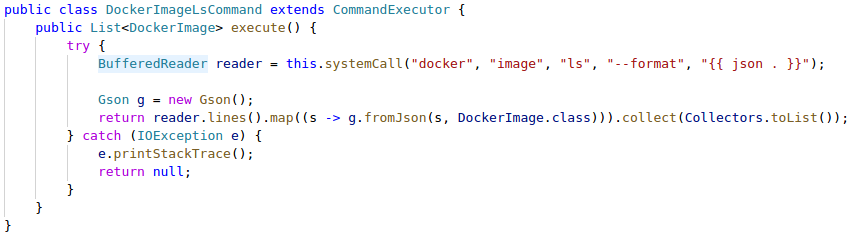
\includegraphics[width=1.0\textwidth]{dockerdriver_dockerimagelscommand}
  \caption{Klass DockerImageLsCommand, mis küsib Dockeri käsurea programmilt süsteemipiltide andmed ja parsib need DockerImage objektideks}
  \label{fig:dockerdriver_dockerimagelscommand}
  \end{center}
  \end{figure}
 
  \FloatBarrier
 
  
  \begin{figure} [ht] %try to place the figure here (next option top of the page) 
  \begin{center}
  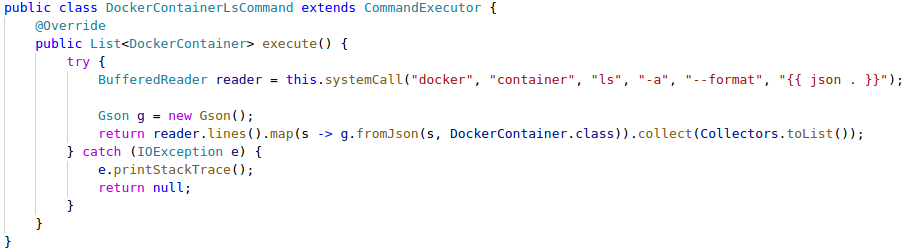
\includegraphics[width=1.0\textwidth]{dockerdriver_dockercontainerlscommand}
  \caption{Klass DockerContainerLsCommand, mis küsib Dockeri käsurea programmilt süsteemipiltide andmed ja parsib need DockerContainer objektideks}
  \label{fig:dockerdriver_dockercontainerlscommand}
  \end{center}
  \end{figure}
 
  \FloatBarrier
  
  Dockeri süsteemipiltide ja konteinerite Cumulocity platvormi saatmise lõpetamiseks on vaja veel defineerida
  DockerDriver klassi ''run'' meetod, mida nõudis PollingDriver klass. Selles küsitakse informatsiooni Dockerilt
  ning see saadetakse Cumulocity andmelattu, mida on näha joonisel \ref{fig:dockerdriver_updatedockerstate}.
  Cumulocity andmelaos Dockeri süsteemipiltide ja konteinerite ühiseks hoiustamiseks loodi Docker nimeline klass,
  mille definitsioon on näha joonisel \ref{fig:dockerdriver_docker}.
 
  \begin{figure} [ht] %try to place the figure here (next option top of the page) 
  \begin{center}
  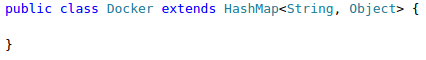
\includegraphics[width=0.7\textwidth]{dockerdriver_docker}
  \caption{Docker klass Dockeri süsteemipiltide ja konteinerite ühiseks hoiustamiseks Cumulocity andmelaos}
  \label{fig:dockerdriver_docker}
  \end{center}
  \end{figure}
 
  \FloatBarrier
 
 
 
  \begin{figure} [ht] %try to place the figure here (next option top of the page) 
  \begin{center}
  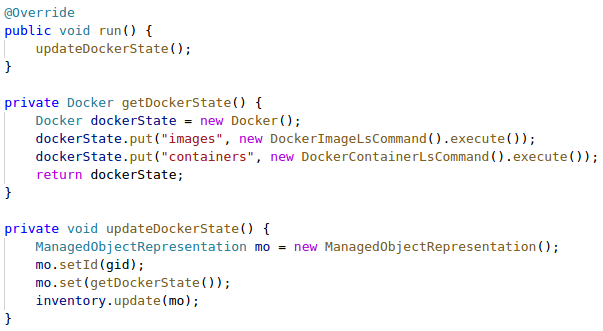
\includegraphics[width=1.0\textwidth]{dockerdriver_updatedockerstate}
  \caption{Meetodid, mille abil saadetakse infot Cumulocity andmelattu seadme Dockeri kohta}
  \label{fig:dockerdriver_updatedockerstate}
  \end{center}
  \end{figure}
 
  \FloatBarrier
 
  
 
   
 %  \begin{figure}
 %   \centering
 %   \begin{minipage}{0.45\textwidth}
 %     \centering
 %     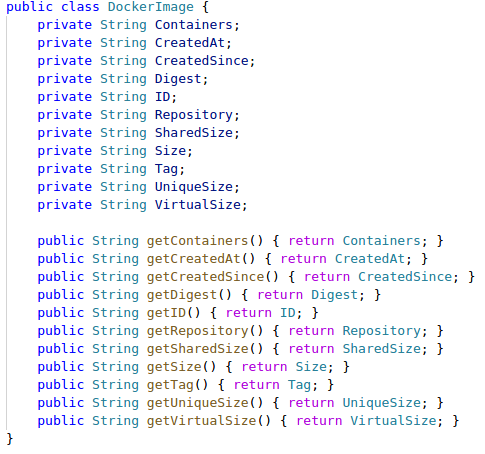
\includegraphics[width=0.9\textwidth]{dockerdriver_dockerimage} % first figure itself
 %     \caption{Klass Dockeri süsteemipiltide hoidmiseks}
 %     \label{fig:dockerdriver_dockerimage}
 %   \end{minipage}\hfill
 %   \begin{minipage}{0.45\textwidth}
 %     \centering
 %     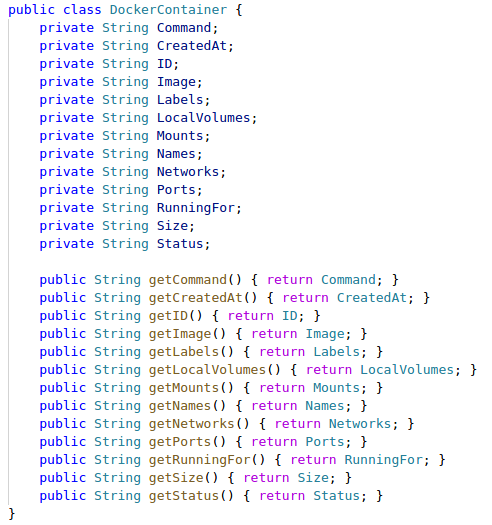
\includegraphics[width=0.9\textwidth]{dockerdriver_dockercontainer} % second figure itself
 %     \caption{Klass Dockeri konteinerite hoidmiseks}
 %     \label{fig:dockerdriver_dockercontainer}
 %   \end{minipage}
 %  \end{figure}
 
 %  \begin{figure} [ht] %try to place the figure here (next option top of the page) 
 %  \begin{center}
 %  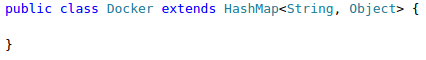
\includegraphics[width=0.6\textwidth]{dockerdriver_docker}
 %  \caption{Klass Dockeri süsteemipiltide ja konteinerite ühiseks hoiustamiseks}
 %  \label{fig:dockerdriver_docker}
 %  \end{center}
 %  \end{figure}
 
  
 %  \FloatBarrier
 
 %  Joonisel \ref{fig:dockerdriver_repository_executecmd} olevast meetodist on tuletatud
 %  DockerRepository klassi sisse meetodid, mille abil saab kätte
 %  seadmel olevad Dockeri süsteemipildid ja konteinerid. 
 
 %  \begin{figure} [ht] %try to place the figure here (next option top of the page) 
 %  \begin{center}
 %  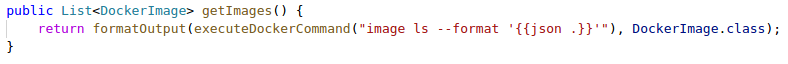
\includegraphics[width=0.9\textwidth]{dockerdriver_repository_getimages}
 %  \caption{Meetod DockerRepository klassis, mis küsib Dockerilt süsteemipildid}
 %  \label{fig:dockerdriver_repository_getimages}
 %  \end{center}
 %  \end{figure}
 
 %  \begin{figure} [ht] %try to place the figure here (next option top of the page) 
 %  \begin{center}
 %  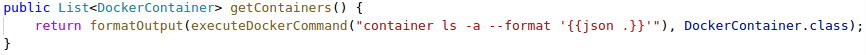
\includegraphics[width=0.9\textwidth]{dockerdriver_repository_getcontainers}
 %  \caption{Meetod DockerRepository klassis, mis küsib Dockerilt konteinerid}
 %  \label{fig:dockerdriver_repository_getcontainers}
 %  \end{center}
 %  \end{figure}
 
 %  \begin{figure} [ht] %try to place the figure here (next option top of the page) 
 %  \begin{center}
 %  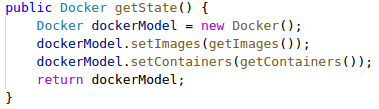
\includegraphics[width=0.4\textwidth]{dockerdriver_repository_getstate}
 %  \caption{Meetod DockerRepository klassis, mis tagastab Dockeri oleku}
 %  \label{fig:dockerdriver_repository_getstate}
 %  \end{center}
 %  \end{figure}
  
 %  \FloatBarrier
  
 %  Dockeri käsurea programmi on nendes käivitatud \verb|"--format '{{json .}}'"| lipuga, kuna 
 %  JSON formaati on lihtne töödelda. Selleks on kasutatud com.google.gson teegist Gson klassi.
 
 %  \begin{figure} [ht] %try to place the figure here (next option top of the page) 
 %  \begin{center}
 %  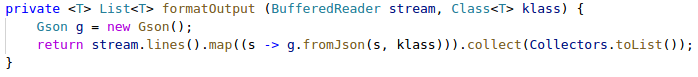
\includegraphics[width=0.9\textwidth]{dockerdriver_repository_formatoutput}
 %  \caption{Meetod DockerRepository klassis, mis formaadib Dockeri käsurea programmi väljundi}
 %  \label{fig:dockerdriver_repository_formatoutput}
 %  \end{center}
 %  \end{figure}
 
 %  \FloatBarrier
  
 %  Mooduli keskmeks on DockerDriver nimeline klass, mille ülemklassiks on\newline
 %  c8y.lx.driver.PollingDriver abstraktne klass, mis pärineb näidiskoodist. See implementeerib
 %  java.lang.Runnable liidest, mistõttu on vaja DockerDriver klassis defineerida "run" meetod.
 %  PollingDriver kutsub seda meetodit ajalise intervalli tagant välja, milleks on
 %  määratud DockerDriver klassis 5 sekundit. Selle meetodi abil saadetakse Cumulocity
 %  andmelattu informatsiooni Dockeri oleku kohta, mis saadakse DockerRepository klassi
 %  getState meetodi abil.
 
 
 
 %  \begin{figure} [ht] %try to place the figure here (next option top of the page) 
 %  \begin{center}
 %  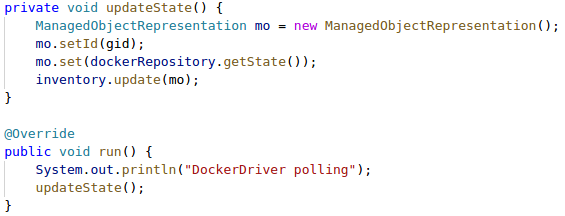
\includegraphics[width=0.8\textwidth]{dockerdriver_run}
 %  \caption{Meetod run DockerDriver klassis, mis saadab informatsiooni Dockeri oleku kohta}
 %  \label{fig:dockerdriver_run}
 %  \end{center}
 %  \end{figure}
  
 %  \FloatBarrier
 
 %  Joonisel \ref{fig:dockerdriver_run} updateState meetodis luuakse uus andmelao objekt
 %  ManagedObjectRepresentation klassi järgi ning selle identifikaatoriks seatakse
 %  praeguse seadme identifikaator. Selle järgi teab Cumulocity andmeladu, millise
 %  seadme juurde see objekt kuulub. Seejärel uuendatakse andmeladu selle objektiga.
 %  Selle tulemusena on seadme Dockeri süsteemipildid ja konteinerid platvormis kätte
 %  saadavad ja veebiliideses kuvatavad.
 
 %  Agendi operatsioonide kuulamine on juba Cumulocity näidisagendis ette defineeritud.
 %  Agent kuulab operatsioonide sündmusi andmelaos, mis sinna läbi API-liidesesse
 %  saadetakse, ja operatsiooni
 %  saabumisel saadetakse see agendi moodulitele laiali. Moodul peab seejärel aru
 %  saama, kas operatsioon oli talle suunatud või mõnele muule moodulile. Kuna agent
 %  agent kuulab kõiki operatsioone andmelaos, siis peab moodul otsustama ka,
 %  kas operatsioon on mõeldud sellele seadmele või mitte.
 
 %  Selleks, et agent teaks, et moodul toetab operatsioonide käivitamist, peab
 %  DockerDriver klass implementeerima c8y.lx.driver.OperationExecutor
 %  liidese, mis nõuab, et moodul teataks oma operatsiooni tüübi,
 %  milleks on ''c8y\_Docker'' nagu joonise
 %  \ref{fig:webplugin_operationsendexample} juures kirjeldatud on. Selleks peab
 %  defineerima kaks meetodit:
 
 %  \begin{figure} [ht] %try to place the figure here (next option top of the page) 
 %  \begin{center}
 %  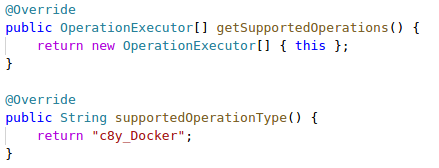
\includegraphics[width=0.6\textwidth]{dockerdriver_supportedoperationtype}
 %  \caption{Meetodid Dockerdriveris, mis teatavad toetatud operatsiooni tüübi agendile}
 %  \label{fig:dockerdriver_supportedoperationtype}
 %  \end{center}
 %  \end{figure}
  
 %  \FloatBarrier
  
 %  OperationExecutor liides ka nõuab ''execute'' meetodi defineerimist. Selles meetodis peab
 %  kontrollima, kas operatsioon on mõeldud sellele seadmele. Veebiliideses saadetud
 %  Dockeri operatsioonid sisaldavad endas ''operationCommand'' muutujat nagu joonise
 %  \ref{fig:webplugin_operationsendexample} juures kirjeldatud on. Selle järgi saab ''execute''
 %  meetodis teada, millist Dockeri käsurea käsku jooksutada. 
 
 %  \begin{figure} [ht] %try to place the figure here (next option top of the page) 
 %  \begin{center}
 %  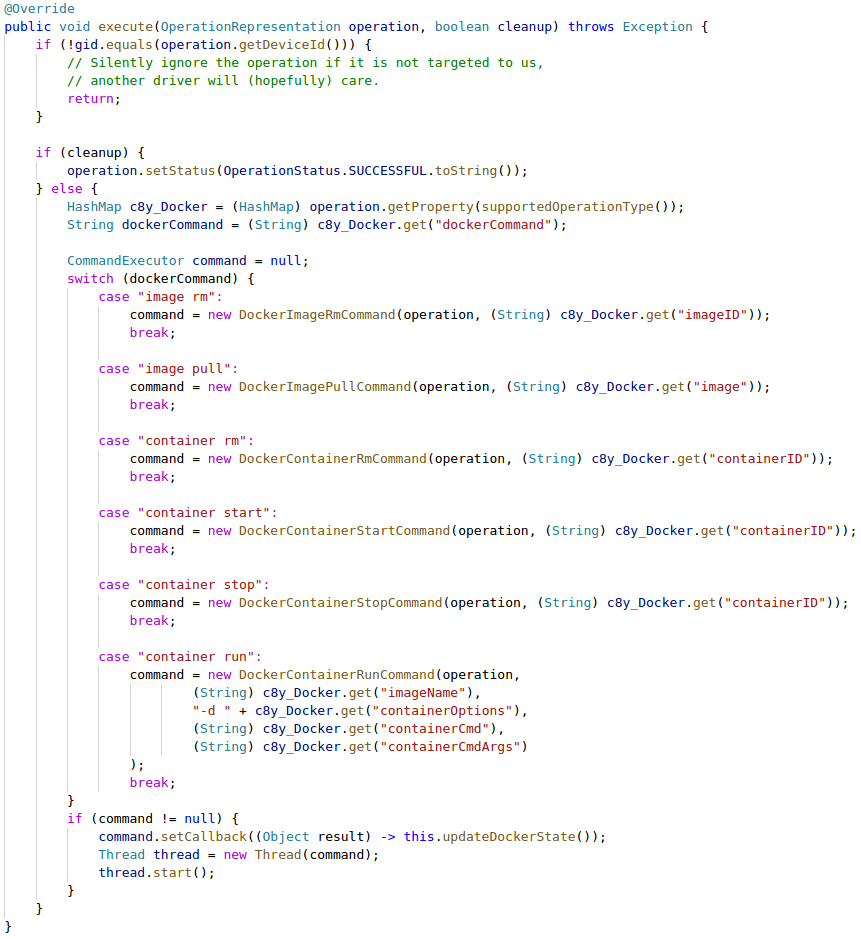
\includegraphics[width=0.8\textwidth]{dockerdriver_execute}
 %  \caption{Meetod execute DockerDriver klassis, mis käivitab vastava Dockeri käsurea programmi sõltuvalt operatsioonist}
 %  \label{fig:dockerdriver_execute}
 %  \end{center}
 %  \end{figure}
 
 %  \FloatBarrier
 
 %  Lõpetuseks vaja täiendada ka DockerRepository klassi süsteemipiltide kustutamise,
 %  konteinerite käivitamise, peatamise, kustutamise ja loomise meetoditega.
 
 %  \begin{figure} [ht] %try to place the figure here (next option top of the page) 
 %  \begin{center}
 %  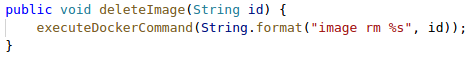
\includegraphics[width=0.7\textwidth]{dockerdriver_repository_deleteimage}
 %  \caption{Meetod DockerRepository klassis, mis käivitab Dockeri käsurea programmi süsteemipiltide kustutamiseks}
 %  \label{fig:dockerdriver_repository_deleteimage}
 %  \end{center}
 %  \end{figure}
 %  \begin{figure} [ht] %try to place the figure here (next option top of the page) 
 %  \begin{center}
 %  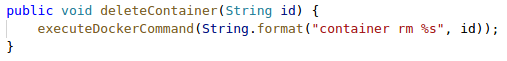
\includegraphics[width=0.7\textwidth]{dockerdriver_repository_deletecontainer}
 %  \caption{Meetod DockerRepository klassis, mis käivitab Dockeri käsurea programmi konteinerite kustutamiseks}
 %  \label{fig:dockerdriver_repository_deletecontainer}
 %  \end{center}
 %  \end{figure}
 %  \begin{figure} [ht] %try to place the figure here (next option top of the page) 
 %  \begin{center}
 %  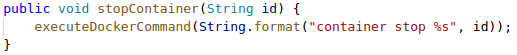
\includegraphics[width=0.7\textwidth]{dockerdriver_repository_stopcontainer}
 %  \caption{Meetod DockerRepository klassis, mis käivitab Dockeri käsurea programmi konteinerite peatamiseks}
 %  \label{fig:dockerdriver_repository_stopcontainer}
 %  \end{center}
 %  \end{figure}
 %  \begin{figure} [h] %try to place the figure here (next option top of the page) 
 %  \begin{center}
 %  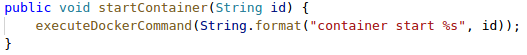
\includegraphics[width=0.7\textwidth]{dockerdriver_repository_startcontainer}
 %  \caption{Meetod DockerRepository klassis, mis käivitab Dockeri käsurea programmi konteinerite käivitamiseks}
 %  \label{fig:dockerdriver_repository_startcontainer}
 %  \end{center}
 %  \end{figure}
 %  \begin{figure} [h] %try to place the figure here (next option top of the page) 
 %  \begin{center}
 %  \includegraphics[width=0.7\textwidth]{dockerdriver_repository_runcontainer}
 %  \caption{Meetod DockerRepository klassis, mis käivitab Dockeri käsurea programmi konteinerite loomiseks}
 %  \label{fig:dockerdriver_repository_runcontainer}
 %  \end{center}
 %  \end{figure}
  
 %  \FloatBarrier
 
 
  \subsection{Lahenduse testimine}
  Lahenduse testimiseks kasutas autor värskelt seadistatud Raspberry Pi seadet, kuna autoril
  oli see seade olemas ning see sobitub hästi
  antud lahenduse kasutuslooga. Seadmele on varasemalt juba Dockeri installeeritud, kasutades
  Dockeri ametlikku installeerimisjuhendit~\cite{DockerInstallDebianGuide}.
  Seadme integreerimiseks platvormiga kõigepealt kompileeriti
  agent kasutades näidisagendi Maveni ''package'' käsku. See genereerib Raspberry Pi jaoks
  ''.deb'' laiendiga paketi, mille abil saab agendi installida. Selleks tuleb see seadmele kopeerida.
  Autor kasutas selle jaoks scp nimelist käsurea programmi, mille abil saab
  faile kopeerida seadmetele üle võrgu~\cite{scp}. Joonisel \ref{fig:scp_usage} on
  demonstreeritud scp programmi kasutamist. Kopeeritav fail ''cumulocity-rpi-agent\_8.19.0\_all.deb''
  asus arendusmasinas ''agent/java-agent/packages/rpi-agent/target/'' kaustas ning see kopeeriti Raspberry Pi
  seadmele, mis asus arendusmasinaga samas võrgus IP-aadressil ''192.168.1.12''. Seadmega ühendus
  tehti läbi ''pi'' kasutaja ning kopeeritava faili lõppasukohaks oli selle kasutaja kodukaust
  Raspberry Pi seadmes(\textasciitilde).
 
  \begin{figure} [ht] %try to place the figure here (next option top of the page) 
  \begin{center}
  \includegraphics[width=1.0\textwidth]{scp_usage}
  \caption{Scp käsurea programmi kasutamine}
  \label{fig:scp_usage}
  \end{center}
  \end{figure}
 
  \FloatBarrier
 
 
  Seejärel installeeriti see fail seadme peale. Selleks tuleb seadmesse sisse logida. Raspberry
  Pi puhul saab seda teha nagu tavalise arvutiga kasutades klaviatuuri, hiirt ja monitori. Autor otsustas
  selle asemel kasutada ssh ühendust, mis võimaldab
  saada seadme käsureale ligipääs üle võrgu~\cite{ssh}. Joonisel \ref{fig:ssh_usage} on logitud arendusmasinaga
  samas võrgus
  IP-aadressil ''192.168.1.12'' olevasse seadmesse ''pi'' nimelisse kasutajasse. Sisse logimisel
  küsitakse ka selle kasutaja parooli, milleks Raspberry Pi seadmel on vaikimisi ''raspberry''.
  
  \begin{figure} [ht] %try to place the figure here (next option top of the page) 
  \begin{center}
  \includegraphics[width=1.0\textwidth]{ssh_usage}
  \caption{Ssh käsurea programmi abil seadmesse logimine}
  \label{fig:ssh_usage}
  \end{center}
  \end{figure}
 
  \FloatBarrier
 
  Ssh ühenduse loomisel antakse ligipääs seadme käsureale, mis on nähtav viimasel real joonisel
  \ref{fig:ssh_usage}. Sealt on näha ka käsurea hetke aktiivne asukoht seadme failisüsteemis, mida markeerib
  peale koolonit olev \textasciitilde, mis tähendab sisselogitud kasutaja kodukausta. See on sama
  kaust, kuhu joonisel \ref{fig:scp_usage} näidatud scp käsk installeerimispaketi kopeeris.
  Joonisel \ref{fig:ls_usage} käsurea programmi ls käivitamine näitab selle faili olemasolu
  praeguses aktiivses failisüsteemi asukohas.
 
  \begin{figure} [ht] %try to place the figure here (next option top of the page) 
  \begin{center}
  \includegraphics[width=1.0\textwidth]{ssh_usage}
  \caption{Käsurea programmiga ls praeguse aktiivse kausta sisu kuvamine.}
  \label{fig:ls_usage}
  \end{center}
  \end{figure}
 
  \FloatBarrier
 
 
  Paketi installeerimiseks kasutati dpkg programmi koos ''--install'' lipuga, mida kujutab
  joonis \ref{fig:dpkg_install}~\cite{dpkg}.
  Kui on soov enne paketi installimist veenduda, mis failid seadmele installitakse, siis saab
  kasutada ''--contents'' lippu, mis tagastab failid ja nende installimisasukohad. Käsku
  jooksutati sudo käsu abil, kuna agent installitakse asukohta, mille sisu muutmiseks on
  vaja administraatori õiguseid.
 
  \begin{figure} [ht] %try to place the figure here (next option top of the page) 
  \begin{center}
  \includegraphics[width=1.0\textwidth]{dpkg_install}
  \caption{Cumulocity agendi installimine dpkg programmi abil}
  \label{fig:dpkg_install}
  \end{center}
  \end{figure}
 
  \FloatBarrier
 
 
  Installi tulemusena kopeeriti paketi seest failid /usr/share/cumulocity-rpi-agent kausta. Selles
  Agent tuleb veel seadistada, et see teaks, millise tenantiga suhelda. Selleks on fail, mille
  asukohaks failisüsteemis on /etc/cumulocity-agent.properties. Faili muutmiseks kasutati
  nano käsurea programmi, mille abil kirjutati faili tenanti url ja nimi. Joonisel
  \ref{fig:agent_configuration} on näha faili sisu peale muutmist.
 
  \begin{figure} [ht] %try to place the figure here (next option top of the page) 
  \begin{center}
  \includegraphics[width=1.0\textwidth]{agent_configuration}
  \caption{Näide Cumulocity agendi seadistusest}
  \label{fig:agent_configuration}
  \end{center}
  \end{figure}
 
  \FloatBarrier
 
 
  Seejärel käivitati agent. Agendi installeerimispakett installeris skripti, läbi mille
  on võimalik agenti käivitada kui teenust. Teenuste haldamiseks on service nimeline käsurea
  programm, mille abil on võimalik teenuseid käivitada, peatada, taaskäivitada ning nende
  olekut vaadata. Agendi käivitamist on näidatud joonisel \ref{fig:agent_service_start}.
  On võimalik, et installimise käigus agent juba käivitati, siis tuleb asendada joonisel
  \ref{fig:agent_service_start} toodud käsus ''start'' sõnaga ''restart''.
 
  \begin{figure} [ht] %try to place the figure here (next option top of the page) 
  \begin{center}
  \includegraphics[width=1.0\textwidth]{agent_service_start}
  \caption{Cumulocity agendi käivitamine teenusena}
  \label{fig:agent_service_start}
  \end{center}
  \end{figure}
 
  \FloatBarrier
 
  Käsu tulemuseks midagi ei väljasta. Seetõttu on kasulik vaadata agendi logi, mille järgi
  saab veenduda, et agent käivitus korralikult ning et mingeid tõrkeid ei tekkinud. Agendi
  logi salvestatakse süsteemi logisse, mis failisüsteemis asub /var/log/syslog asukohas.
  
  Seadme registreerimise lõpetamiseks lisati Cumulocity veebikeskkonnas seadmehaldus
  rakenduse alt registreerimisvaatesse kirje uue seadme kohta. Kirje nõuab seadme ID väärtust,
  milleks seadme seerianumber. Raspberry Pi puhul on see nähtav /proc/cpuinfo failist, mille
  lõpus on kirje ''Serial'', millele järgneb numbritest ja tähtedest koosnev jada. See jada
  tuleb sisestati veebikeskkonda. Seepeale lubab Cumulocity seadmel platvormiga ühenduda ning
  seadmel olev agent saadab seadme kohta andmed. Seejärel kinnitati veebikeskkonnas
  seadme õigsust, millega seadme registreerimine lõppeb. Seade ilmub Cumulocity veebikeskkonnas
  seadmehaldus rakenduse all kõigi seadmete vaatesse.
 
  Dockeri konteinerite ja süsteemipiltide vaadete tabelid on tühjad, kuna seadmes ei ole
  ühtegi süsteemipilti ega konteinerit veel (Joonis \ref{fig:test_noimages} ja
  \ref{fig:test_nocontainers}).
 
  \begin{figure} [ht] %try to place the figure here (next option top of the page) 
  \begin{center}
  \includegraphics[width=1.0\textwidth]{test_nocontainers}
  \caption{Konteinerite vaade testimisseadmel}
  \label{fig:test_nocontainers}
  \end{center}
  \end{figure}
 
  \FloatBarrier
  
  \begin{figure} [ht] %try to place the figure here (next option top of the page) 
  \begin{center}
  \includegraphics[width=1.0\textwidth]{test_noimages}
  \caption{Süsteemipiltide vaade testimisseadmel}
  \label{fig:test_noimages}
  \end{center}
  \end{figure}
 
  \FloatBarrier
 
 
  Testimiseks kasutati nginx:latest nimelist süsteemipilti, mis sisaldab endas Nginx\footnote{https://www.nginx.com/}
  veebiserveri tarkvara. See on vabalt kättesaadav ning kuna tegemist on veebiserveriga, mis töötab pordil 80,
  siis on võimalik
  selle töötamist seadmel valideerida curl käsu abil. Süsteemipildi allalaadimiseks kasutati süsteemipiltide
  vaates ''Pull image'' alamsektsiooni, kuhu sisestati ''nginx:latest''. Kuna süsteemipilt tuleb alla
  laadida, siis sõltuvalt internetiühenduse kiirusest on allalaadimiseks kuluv aeg erinev. Siis uuendati
  vaadet kasutades ''reload'' nuppu vaate paremal üleval nurgas, mida on näha jooniselt \ref{fig:test_noimages}.
  Süsteemipilt nginx:latest ilmus süsteemipiltide vaates olevasse tabelisse.
 
  Järgnevalt loodi sellest süsteemipildist konteiner, kasutades konteinerite vaates olevat ''Create container''
  alamsektsiooni. Süsteemipildiks valiti nginx:latest ning ''run options'' väljale sisestati
  \verb|--publish 80:80|, et siduda seadme port 80 konteineri pordiga 80. See tagab, et
  konteineris töötav veebiserver oleks kättesaadav väljaspool konteinerit.
  Seejärel vajutati ''Create'' nuppu ja uuendati vaadet
  ''reload'' nupuga. Tulemusena ilmus konteinerite vaates tabelisse aktiivne konteiner
  (Joonis \ref{fig:test_activecontainer}).
 
  \begin{figure} [ht] %try to place the figure here (next option top of the page) 
  \begin{center}
  \includegraphics[width=1.0\textwidth]{test_activecontainer}
  \caption{Aktiivne Dockeri konteiner töötamas Raspberry Pi seadmel}
  \label{fig:test_activecontainer}
  \end{center}
  \end{figure}
 
  \FloatBarrier
 
  
  Konteineris jooksva veebiserveri ligipääsu testimiseks tehti curl käsurea programmi abil
  GET päring vastu seadme port 80, mis on nähtav jooniselt \ref{fig:test_curlactive}. Tulemusena
  tagastati tervitussõnum, mis tähendab, et konteineris veebiserver tõepoolest töötab ning
  see on seadme pordilt 80 kättesaadav.
 
  \begin{figure} [ht] %try to place the figure here (next option top of the page) 
  \begin{center}
  \includegraphics[width=1.0\textwidth]{test_curlactive}
  \caption{Raspberry Pi seadmele tehtud päring konteineris töötava veebiserveri valideerimiseks}
  \label{fig:test_curlactive}
  \end{center}
  \end{figure}
 
  \FloatBarrier
 
  Seejärel konteiner peatati, uuendati vaadet ning tabelis muutus äsja aktiivne olnud konteineri
  roheline tagataust valgeks. Sama konteiner uuesti käivitades muutus taust uuesti roheliseks.
  Konteineri kustutamiseks peatati konteiner uuesti ning seejärel kustutati konteiner. Tabelit
  uuendades kadus konteiner tabelist ja konteinerite tabeli seis on samasugune nagu joonisel \ref{fig:test_nocontainers}.
  Seejärel kustutati nginx:latest süsteemipilt ja süsteemipiltide tabeli seisu tulemus on sama nagu
  joonisel \ref{fig:test_noimages}.
 
  Sellega on valideeritud uue tarkvara allalaadimine Dockeri süsteemipildina, sellest konteineri loomine
  koos konteinerile argumentide täpsustamisega, konteineri peatamine, käivitamine ja kustutamine ning
  süsteemipildi kustutamine.
 
 
  
  
  
  
 
 
 
 
  \subsection{Edasiarendused}
  Veebiliidese moodulis peab hetkel manuaalselt uuendama Dockeri konteinereid ja süsteemipilte
  tabelites. Kasutajamugavuse poolest oleks hea, kui need uuendused toimuksid reaalajas ning
  kasutaja ei peaks ''reload'' nuppu vajutama peale igat operatsiooni. Samuti võiksid esineda
  abitekstid, mis tutvustaksid liidest esmakordsele kasutajale.
  Seadmele operatsioonide
  saatmise puhul ei uuenda agent automaatselt operatsioonide staatust ''successful'' olekusse,
  kuna operatsioonide delegeerimine moodulitesse ning nende käivitamine toimub agendi poole pealt
  sünkroonselt, kuid operatsiooni sisene tegevus on asünkroone.
  Liideses on implementeeritud põhilised Dockeri funktsioonid, aga liidest on võimalik arenendada
  neid uusi funktsioone lisades. Näiteks lisada Dockeri volüümide või võrkude haldamine.
 
 
 
 
 
 
 
 
 
  \clearpage
  \section{Kokkuvõte}
  Käesoleva bakalaureusetöö eesmärgiks oli luua liides, mis ühendab omavahel Cumulocity platvormi
  ja Dockeri. Liides pidi võimaldama saada ülevaadet Dockeri süsteemipiltide ja konteinerite kohta.
  Süsteemipilte olema võimalik ka kustutada ning konteinereid pidi saama käivitada, peatada, kustudada
  ja uusi luua. 
 
  Töö raames valmis Angular.js raamistikul põhinev Cumulocity veebiliidese moodul, mis suhtleb Cumulocity
  API-liidesega, küsides Cumulocity andmelaost andmeid seadme Dockeri süsteemipiltide ja konteinerite kohta.
  Moodul oskab neid kuvada ülejäänud veebiliidesega sarnases stiilis. Samuti võimaldab moodul
  saata Dockeri põhiseid operatsioone.
  Seadmele loodi agent, mis saadab iga 5 sekundi tagant andmeid Dockeri süsteemipiltide ja konteinerite kohta.
  Agent oskab kuulata Cumulocity andmelattu saabuvaid operatsioone ning vastavalt nendele
  käivitada Dockeri käsurea programmi süsteemipiltide ja konteinerite haldamiseks.
 
  Cumulocity platvorm on väga paindlik tööriist, mis võimaldab omavahel integreerida erinevaid
  tehnoloogaid, mis teevad asjade interneti seadmete haldamise lihtsaks. Kui Cumulocityga seotud seade on võimeline
  Dockeri konteinereid jooksutama, siis loodav agent võimaldab seadmel olevat tarkvara reaalajas hallata otse
  Cumulocity veebiliidese kaudu. Kõike seda saab teha läbi brauseri ja tänu Cumulocityle on võimalik hallata
  Dockeri konteinerite kaudu töötavat tarkvara mitmetes seadmetes samaaegselt. Selle kasu on eriti näha
  asjade interneti seadmetes, kuna suurtes süsteemides muutub nende tarkvara haldamine keeruliseks.
  Loodud lahendus, mis ühendab omavahel Dockeri ja Cumulocity platvormi, on autori teades ainulaadne.
 
  Varasemalt oli töö autoril väikene kokkupuude Dockeriga ning selle konteinerite ja süsteemipiltidega.
  Cumulocity platvormiga kokkupuude oli esmakordne ja see oli töö juures kõige keerulisem osa.
  
  
  
 
 
  \newpage
  
  % BibTeX bibliography
  % \bibliographystyle{alpha} %plain=[1], alpha=[BGZ09]
  \bibliographystyle{plain}
  \bibliography{docker}
  
  \addcontentsline{toc}{section}{\refname}
   
   
 
  \newpage
  \section*{Lisad}
  \addcontentsline{toc}{section}{Lisad}
   
  \section*{I. Lahenduse repositoorium}
  \addcontentsline{toc}{subsection}{I. Lahenduse repositoorium}
  \label{sec:lisa_lahenduserepo}
  Autori poolt loodud lahendus on kättesaadav Githubi repositooriumist, mis asub aadressil
  \url{https://github.com/marcus17777/bachelor_thesis}. Kaustas ''agent'' leidub Cumulocity
  näidisagendil põhinev agent, mis sisaldab endas docker-driver nimelist moodulit, mis vastutab
  Dockeri süsteemipiltide ja konteinerite halduse eest. Kaustas ''webplugin'' asub Cumulocity 
  veebiliidese moodul. Repositooriumist on kättesaadav ka see sama dokument ja LaTeX
  allikas, mille põhjal see dokument loodi.
  



  \newpage
  
  %=== Licence in English
  \newcommand\EngLicence{{%
  \selectlanguage{english}
  \section*{II. Licence}
  
  \addcontentsline{toc}{subsection}{II. Licence}
  
  \subsection*{Non-exclusive licence to reproduce thesis and make thesis public}
  
  I, \textbf{Markus Peterson},
  
  \begin{enumerate}
  \item
  herewith grant the University of Tartu a free permit (non-exclusive licence) to:
  \begin{enumerate}
  \item[1.1]
  reproduce, for the purpose of preservation and making available to the public, including for addition to the DSpace digital archives until expiry of the term of validity of the copyright, and
  \item[1.2]
  make available to the public via the web environment of the University of Tartu, including via the DSpace digital archives until expiry of the term of validity of the copyright,
  \end{enumerate}
  
  of my thesis
  
  \textbf{Remote management of Docker containers in IoT device}
  
  supervised by Pelle Jakovits
  
  \item
  I am aware of the fact that the author retains these rights.
  \item
  I certify that granting the non-exclusive licence does not infringe the intellectual property rights or rights arising from the Personal Data Protection Act. 
  \end{enumerate}
  
  \noindent
  Tartu, 14.05.2018
  }}%\newcommand\EngLicence
  
  
  %=== Licence in Estonian
  \newcommand\EstLicence{{%
  \selectlanguage{estonian}
  \section*{II. Litsents}
  
  \addcontentsline{toc}{subsection}{II. Litsents}
  
  \subsection*{Lihtlitsents lõputöö reprodutseerimiseks ja lõputöö üldsusele kättesaadavaks tegemiseks}
  
  Mina, \textbf{Markus Peterson},
  
  \begin{enumerate}
  \item
  annan Tartu Ülikoolile tasuta loa (lihtlitsentsi) enda loodud teose
  
  \textbf{Dockeri konteinerite kaughaldus IoT seadmetes}
  
  mille juhendaja on Pelle Jakovits
  
  \begin{enumerate}
  \item[1.1]
  reprodutseerimiseks säilitamise ja üldsusele kättesaadavaks tegemise eesmärgil, sealhulgas digitaalarhiivi DSpace-is lisamise eesmärgil kuni autoriõiguse kehtivuse tähtaja lõppemiseni;
  \item[1.2]
  üldsusele kättesaadavaks tegemiseks Tartu Ülikooli veebikeskkonna kaudu, sealhulgas digitaalarhiivi DSpace´i kaudu kuni autoriõiguse kehtivuse tähtaja lõppemiseni.
  \end{enumerate}
  
  
  \item
  olen teadlik, et punktis 1 nimetatud õigused jäävad alles ka autorile.
  \item
  kinnitan, et lihtlitsentsi andmisega ei rikuta teiste isikute intellektuaalomandi ega isikuandmete kaitse seadusest tulenevaid õigusi. 
  \end{enumerate}
  
  \noindent
  Tartus, 27.05.2018
  }}%\newcommand\EstLicence
  
  
  %===Choose the licence in active language
  \EstLicence
  
  
  \end{document}
